\documentclass[a4paper, 12pt]{report}
\usepackage[top=2.5cm,bottom=2.5cm,left=2.5cm,right=2.5cm]{geometry}
%-----------------------------------------------------------------------  01
\usepackage[pdftex]{graphicx}
\usepackage{graphics}
\usepackage{fancyhdr} 
%----------------------------------------------------------------------   02
\usepackage[utf8]{inputenc} 
\usepackage[T1]{fontenc}
\usepackage[french]{babel}
\usepackage{array}

\usepackage{makecell, amssymb, amsthm, mathtools, rotating, colortbl, enumitem, nomencl, latexsym, bookmark, url, subcaption, float, multirow, algorithm, algorithmic, color}
\usepackage{arabtex, utf8}
\setcode{utf8}
\usepackage[nomain, acronym]{glossaries}

%-----------------------------------------------------------------------   03
\linespread{1.5}


\begin{document} 
	\begin{titlepage}
		%------------------------------------------------------------------------  04
		\begin{figure}[htbp]
			\hbox{
				\hspace*{-1.4cm}
				
\includegraphics[width=100px]{/home/mohamed/mes_fichier/CADORIM/LaTeX/pfe/Template LaTeX/Images/ISCAE.jpg}
				\hspace*{11cm}
				
\includegraphics[width=80px]{/home/mohamed/mes_fichier/CADORIM/LaTeX/pfe/Template LaTeX/Images/logoUniv.jpg}
			}
		\end{figure}
		%-------------------------------------------------------------------------- 05
		\vspace {-4cm}
		
		\begin{center}
			\vspace{1cm}
			
			{\bf République Islamique de Mauritanie } \vspace{-0.2cm}\\
			{\bf	Ministre de l’Enseignement Supérieur et de la } \vspace{-0.2cm}\\
			
			{\bf Recherche Scientifique }\\
			
			\vspace{2cm}
			
			%------------------------------------------------------------------------- 06
			\bf{MÉMOIRE DE STAGE DE FIN D'ÉTUDES} \\
			\vspace{1cm}
			{\bf Présenté en vue de l’obtention du } \vspace{-0.2cm}\\
			{\bf Diplôme de Master Professionnel en Informatique}\vspace{-0.2cm}\\
				{\bf	Appliquée à la Gestion (MPIAG)}\\ \vspace{0.2cm}
				{\bf Par :}\\ \vspace{0.2cm}
					{\bf Mohamed Lemine Salem M’bedah (IE18689) }\\ \vspace{0.2cm}
			\huge{\textbf{Thème}}\\ 
			\noindent\rule{\textwidth}{1mm}
			\Large{\bf{CREATION D’UN SYSTEME DE GESTION DE RELATION CLIENT (CRM)  ET DE KYC  \\ (KNOW YOUR CUSTOMER)}}
			\noindent\rule{\textwidth}{1mm}
		\end{center}
		\vspace{0cm}
		%-------------------------------------------------------------------------- 07
		\begin{center}
			
			{\bf Encadré par :}\\
			{Dr. Cheikh Dhib} \\
			{Mr. Mboirick Mohamed} \\
			{\bf Réalisé au sein de CADORIM }
			
			
		\end{center}
		\begin{figure}[htbp]
		\hbox{
			\hspace*{5cm}
			
\includegraphics[width=150px]{/home/mohamed/mes_fichier/CADORIM/LaTeX/pfe/Template LaTeX/Images/cado_logo.png}
		} 
		\end{figure}
		
		\begin{center}
			Année universitaire 2021-2022
		\end{center}
		%--------------------------------------------------------------------------- 08
	\end{titlepage}
		\chapter*{DEDICACES} \label{chap:1Dedicaces}
		\addcontentsline{toc}{chapter}{DEDICACES} 
		Les mots ne sauront traduire ce qui est dans le cœur, mais je vais rassembler mon vocabulaire et dire : je dédie cet humble travail à mes chers parents pour leur soutien tout au long de mon parcours universitaire, qui ont été les encouragements dans les moments de détresse, l'exhortation en période de prospérité, le soutien lors de la chute et le guide lors de la montée, qui n'a pas hésité un instant à m'aider jusqu'à ce que j'ai arrivé là où je suis maintenant. Tous les remerciements et gratitudes ne remplissent pas leur droit.
		%sa signification
			%\textbf{<< Dis, mon Seigneur, aie pitié d'eux comme ils m'ont élevé quand j'étais jeune >>}
		\thispagestyle{empty} 
		\chapter*{REMERCIEMENTS} \label{chap:1REMERCIEMENTS}
		\addcontentsline{toc}{chapter}{REMERCIEMENTS} 
		\textit{
			Ce n’est pas parce que la tradition l’exige que cette page se trouve dans ce rapport, mais par ce que les gens à qui s’adressent mes remerciements les méritent vraiment.
			\newline
			J’adresse mes remerciements les plus chaleureux envers : 
			\begin{enumerate}
				 \item[•] \textbf{Dr. Cheikh Dhib,} l'ancien coordinateur de MPIAG, ainsi que \textbf{Dr. Emani Mohamed Sidi} le nouveau coordinateur et l’ensemble du corps
				 professoral et administratif de l’ISCAE.
				 Et pour avoir suivi et dirigé l’évolution de mon travail, ainsi que les encouragements, conseils et orientations réguliers qu’il m’a prodigué.
				 Je vous suis infiniment reconnaissant pour votre grande disponibilité et l’intérêt que vous avez porté à ce travail;
				  \item[•] \textbf{Mr. Mboirick Mohamed, } responsable technique et mon maître de stage, pour sa disponibilité, sa gentillesse, son attention particulière à l’égard de ce travail.
				  Et pour avoir mis les moyens nécessaires au bon déroulement de ce stage de six mois et à la réalisation de ce travail;
				  Je vous suis infiniment reconnaissant pour votre grande disponibilité et l’intérêt que vous avez porté à ce travail;
			\end{enumerate}
			Toutes les personnes qui de près ou de loin, ont contribué à la réalisation de ce travail.
		 }
	 \thispagestyle{empty}
	 \chapter*{AVANT-PROPOS} \label{chap:1AVANT-PROPOS}
	\addcontentsline{toc}{chapter}{AVANT-PROPOS}
	L’Institut Supérieur de Comptabilité et d’Administration des Entreprises est un établissement public d’enseignement supérieur et de recherche, placé sous la tutelle du Ministère en charge de l’Enseignement Supérieur, crée en 2009, par décret N° 2009-161 du 29 avril 2009.
	\newline
	L’ISCAE compte deux (2) départements et dans le cadre de leur formation, les étudiants qui sont en fin de cycle sont tenus d’effectuer un stage pratique au sein d’une entreprise ou d’un service informatique.
	\thispagestyle{empty}
	\chapter*{RESUME} \label{chap:1Resumé}
	\addcontentsline{toc}{chapter}{RESUME}
	Ce document présente les travails suivants :
	\begin{enumerate}
		\item Mise en place d’un système d’extration des donnees à partir des images et traitement des ces donnees.
		\item Elaboration d’un système de verificitation des donners KYC pour lutter contre les fraudes a la carte bancaire.
		\item Tracking de l’activite d’un client sur une application.
		\item Mise en place d’un système de messagerie instantané ( Live chat ).
		\item Système pour suivre les demandes de clients, de la soumission juqu’au traitement et l’archivage.
		\item Mise en place d’un système de repporting et de monitoring.
		\item Mise en place d’un système de notification automatique.
		\item La documention.
	\end{enumerate}
	\thispagestyle{empty}
	\chapter*{LISTE DES ABRÉVIATIONS} \label{chap:1SIGLES ET ABREVIATIONS}
	\addcontentsline{toc}{chapter}{SIGLES ET ABREVIATIONS}
	Je présente ici certains sigles et abréviations que nous utiliserons dans le document.
	\newline\newline
	\textbf{ISCAE} : Institut Supérieur de Comptabilité et d’Administration des Entreprises \newline
	\textbf{MPIAG} : Master Professionnel en Informatique Appliquée à la Gestion \newline
	\textbf{API} : Application Programming Interface \newline
	\textbf{MVC} : Modèle Vue Contrôleur \newline
	\textbf{HTTP} : Hypertext Transfer Protocol \newline
	\textbf{HTTPS} : HyperText Transfer Protocol Secure \newline
	\textbf{UML} : Unified Modeling Language \newline
	\textbf{SQL} : Structured Query Language \newline
	\textbf{JSON} : JavaScript Object Notation \newline
	\textbf{XP} : eXtreme Programming \newline
	\textbf{IIS} : Internet Information Services \newline
	\textbf{DAO} : Data Access Object \newline
	\textbf{AAB} : Android App Bundles \newline
	\textbf{APK} : Android Package Kit \newline
	\textbf{IDE} : Integrated Development Environment (Environnement de Développement Intégré) \newline
	\textbf{MERISE} : Méthode d’Étude et de Réalisation Informatique par les Sous-Ensembles ou pour les Systèmes d’Entreprise \newline
	\textbf{OPT} : One-Time Password \newline
	\textbf{SGBD} : Système de Gestion de Bases de Données \newline
	\textbf{SGBDR} : Système de Gestion de Bases de Données Relationnelle \newline
	\textbf{SOA} : Service Oriented Architecture \newline
	\textbf{OCR} : Optical Character Recognition  \newline 
	\textbf{MRZ} : Machine-Readable Zone  \newline 
	\thispagestyle{empty}
	\tableofcontents
	\let\cleardoublepage\clearpage

\chapter{Introduction générale}
\label{sec:DescriptionDuProjet}

Savoir qui est votre client et adopter des protocoles pour prévenir la criminalité financière sont des défis permanents pour les institutions financières. De manière significative, les institutions financières (y compris les banques, les coopératives de crédit et les sociétés financières du Fortune 50) doivent se conformer à un ensemble de réglementations de plus en plus complexes pour la vérification de l'identité des clients appelée KYC.

KYC, également connu sous le nom de "Know Your Customer" ou "Know Your Client", est un ensemble de procédures permettant de vérifier l'identité d'un client avant ou pendant les transactions avec les banques et autres institutions financières. Le respect des réglementations KYC peut aider à tenir à distance le blanchiment d'argent, le financement du terrorisme et d'autres stratagèmes de fraude courants. En vérifiant d'abord l'identité et les intentions d'un client au moment de l'ouverture du compte, puis en comprenant ses habitudes de transaction, les institutions financières sont en mesure d'identifier plus précisément les activités suspectes. 

Les institutions financières sont soumises à des normes de plus en plus strictes en matière de lois KYC. Ils doivent dépenser plus d'argent pour se conformer à KYC ou être passibles de lourdes amendes. Ces réglementations signifient que presque toutes les entreprises, plateformes ou organisations qui interagissent avec une institution financière pour ouvrir un compte ou effectuer des transactions devront se conformer à ces obligations.

La gestion de la relation client (CRM) est la combinaison de pratiques, de stratégies et de technologies que les entreprises utilisent pour gérer et analyser les interactions et les données client tout au long du cycle de vie du client. L'objectif est d'améliorer les relations de service client, de contribuer à la fidélisation de la clientèle et de stimuler la croissance des ventes. Les systèmes CRM compilent les données client à travers différents canaux, ou points de contact, entre le client et l'entreprise, qui peuvent inclure le site Web de l'entreprise, le téléphone, le chat en direct, le publipostage, les supports marketing et les réseaux sociaux. Les systèmes CRM peuvent également donner aux membres du personnel en contact avec les clients des informations détaillées sur les informations personnelles des clients, l'historique des achats, les préférences et les préoccupations d'achat.


\section{Motivations}

KYC est un moyen de rendre la vérification de l'identité des clients plus précise et moins vulnérable à la fraude.

KYC doivent être effectuées lors de l'intégration d'un nouveau client, mais il est préférable de répéter ces vérifications de temps en temps, pour s'assurer que tout est comme il se doit. En surveillant les comptes clients de cette manière, les comportements suspects peuvent être signalés plus rapidement.

Un système CRM fournit des flux de travail automatisés qui permettent à votre équipe marketing de consacrer plus de temps à des tâches stratégiques, telles que la création de campagnes marketing qui résonnent, l'analyse des données de ces campagnes et le test de différentes approches basées sur ces analyses. Les agents du service client peuvent passer leur temps à travailler avec des clients qui ont des questions, des problèmes ou des besoins plus complexes. En bref, avec des processus de service client plus efficaces, les entreprises peuvent établir de meilleures relations avec leurs clients.

\section{Problématiques}

En réalité, la réalisation d'une application,qui applique le principe de KYC et integre un  système CRM,
nécessite
de faire face à des problématiques diverses et complexes. Ainsi, la société a décidé de se contenter,
dans un premier temps, Mise en place d’un système d’extration des donnees à partir des images et traitement des ces donnees(carte d'identité ou passeport).
Ce sujet soulève de nombreuses questions aux implications différentes. Comment peut extraire le texte apartir de l'image? Comment sera-t-il traité ? Comment peut-il être utilisé dans le principe KYC ? Comment pouvons-nous obtenir un système CRM intégré ?


\section{Objectifs}

La mise en place d'une application pour appliquer l'ide de KYC en basant sur les différent technologie disponible . En basan sur l'extraction du text apartir d'une imange OCR on peut extracter la code MRZ apartir d'une imange du piece d'idendite ou passport est passe le code a un algorithem qui permer de d'etecter les information personnel.



	\chapter{Contexte général du projet}
%\chapter{Présentation de l’entreprise}
\label{chap:introduction}
\section{Présentation du lieu de stage}
%\pagenumbering{arabic}
\subsection{Introduction}
\begin{figure}[h]
	
\includegraphics[scale=0.14]{./Template LaTeX/Images/cado_logo.png}
	\centering
	\caption{CADOROM}
\end{figure}
CADORIM est une société de transfert d’argent mauritanienne basée à Nouakchott,
fondée fin 2018 par un entrepreneur mauritanien, titulaire d'un doctorat en
mathématiques,
CADORIM consiste a transférer de l’argent depuis n’importe quel pays dans le
monde vers ses proches en Mauritanie. Notre objectif et de fourni une plateforme
numérique permet à l’utilisateur de régler ses commandes en toute sécurité et
confidentialité assurée par le service de PayPal qui est mondialement connu pour sa
fiabilité et simplicité.t Pour effectuer un paiement il suffit d'une simple carte bancaire
ou un compte PayPal . et une éventuelle possibilité de virement bancaire.
CADORIM a été élu comme le champion de Banque Centrale de Mauritanie (BCM )
1ère édition 2019 Fintech Challenge,
Le siège social de CADORIM est situé à marche capital , Nouakchott, Mauritanie,
immatriculée au registre du commerce.
\subsection{Missions}
CADORIM offre une large palette de prestations organisées autour des activités suivantes :
\begin{enumerate}
	
	\item Maintenance et amélioration de leurs propres applications (CadoRim et MauriPay)
	\item Développement des applications 
	\item Des agences des reçoivent d'argent et de service client
	
\end{enumerate}
\subsection{Organigramme}
La structure organisationnelle de CADORIM comprend :
\begin{figure}[h]
	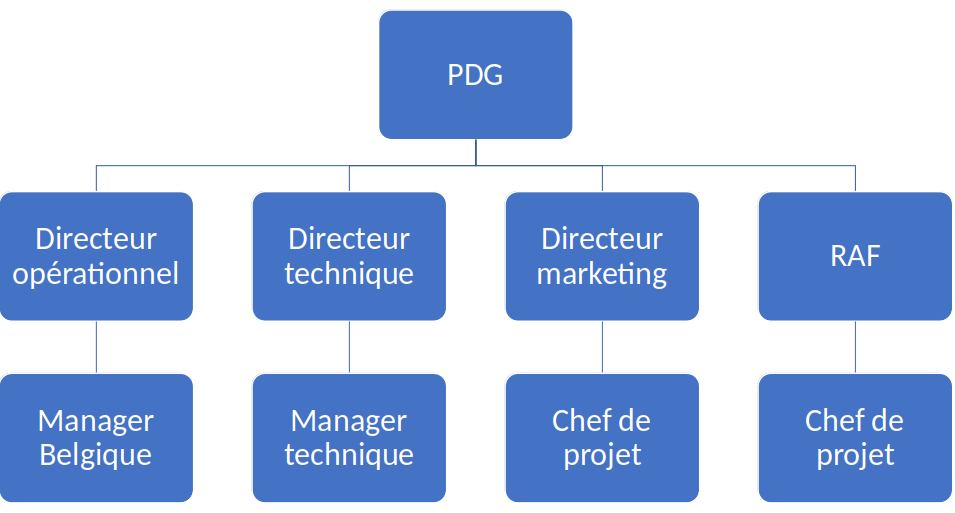
\includegraphics[scale=0.8,width=400px]{./Template LaTeX/Images/og.png}
	\centering
	\caption{Organigramme du CADORIM}
\end{figure}
\begin{comment}
	content...

\subsection{Planification du projet}
J'effectuais le diagramme de Gantt, pour avoir une meilleure compréhension de la chronologie des étapes de mon projet.
\newline
\newline
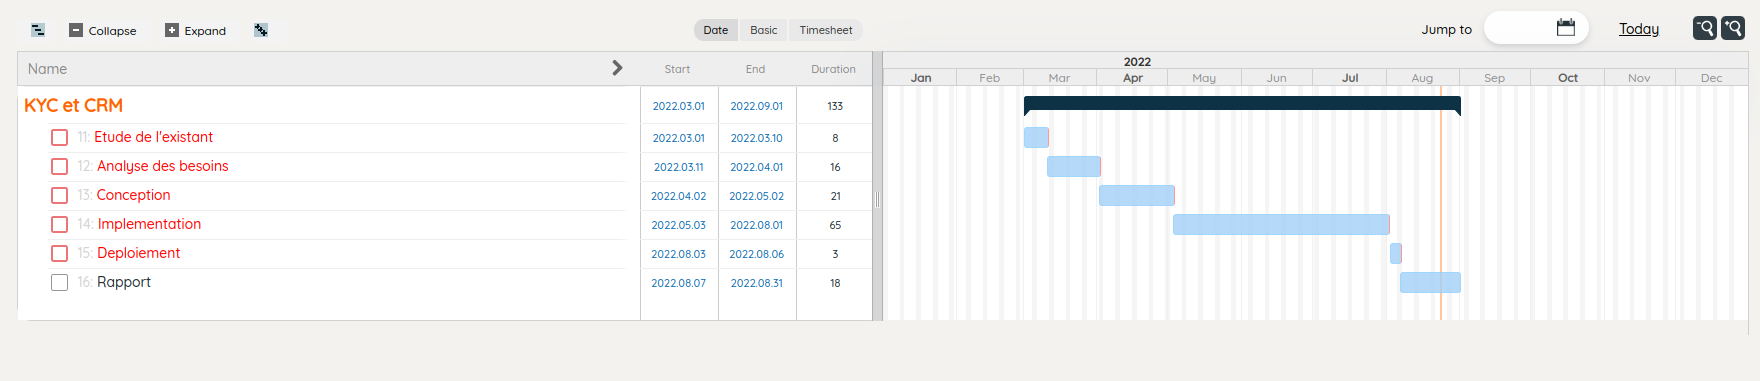
\includegraphics[width=500px,height=175px]{./Template LaTeX/Images/gantt.png}
\newline
Le projet est subdivisé en plusieurs phases.
\begin{enumerate}
\item Une phase comprenant l’étude de l’existant et analyse des besoins, en
intervenant les différents acteurs du projet.
\item Une phase de conception consistant à modéliser et formaliser les
données brutes du cahier de charge
\item Une phase d’implémentation consiste à traduire techniquement les
données provenant de la conception.
\item Déploiement : externalisation des ressources.
\end{enumerate}
\end{comment}
\newpage
\section{Description du projet}
%%%%%%%%%%%%%%%%%%%%%%%%%%%%%%%%%%%%% New add from Introduction %%%%%%%%%%%%%%%%%%%%%
\begin{comment}
	content...

Savoir qui est votre client et adopter des protocoles pour prévenir la criminalité financière sont des défis permanents pour les institutions financières. De manière significative, les institutions financières (y compris les banques, les coopératives de crédit et les sociétés financières du Fortune 50) doivent se conformer à un ensemble des réglementations de plus en plus complexes pour la vérification de l'identité des clients appelée KYC.

KYC, également connu sous le nom de "Know Your Customer" ou "Know Your Client", est un ensemble de procédures permettant de vérifier l'identité d'un client avant ou pendant les transactions avec les banques et autres institutions financières. Le respect des réglementations KYC peut aider à tenir à distance le blanchiment d'argent, le financement du terrorisme et d'autres stratagèmes de fraude courants. En vérifiant d'abord l'identité et les intentions d'un client au moment de l'ouverture du compte, puis en comprenant ses habitudes de transaction, les institutions financières sont en mesure d'identifier plus précisément les activités suspectes. 

Les institutions financières sont soumises à des normes de plus en plus strictes en matière de lois KYC. Ils doivent dépenser plus d'argent pour se conformer à KYC ou être passibles de lourdes amendes. Ces réglementations signifient que presque toutes les entreprises, plateformes ou organisations qui interagissent avec une institution financière pour ouvrir un compte ou effectuer des transactions devront se conformer à ces obligations.

La gestion de la relation client (CRM) est la combinaison de pratiques, de stratégies et de technologies que les entreprises utilisent pour gérer et analyser les interactions et les données client tout au long du cycle de vie du client. L'objectif est d'améliorer les relations de service client, de contribuer à la fidélisation de la clientèle et de stimuler la croissance des ventes. Les systèmes CRM compilent les données client à travers différents canaux, ou points de contact, entre le client et l'entreprise, qui peuvent inclure le site Web de l'entreprise, le téléphone, le chat en direct, le publipostage, les supports marketing et les réseaux sociaux. Les systèmes CRM peuvent également donner aux membres du personnel en contact avec les clients des informations détaillées sur les informations personnelles des clients, l'historique des achats, les préférences et les préoccupations d'achat.


\subsection{Motivations}    

KYC est un moyen de rendre la vérification de l'identité des clients plus précise et moins vulnérable à la fraude.

KYC doivent être effectuées lors de l'intégration d'un nouveau client, mais il est préférable de répéter ces vérifications de temps en temps, pour s'assurer que tout est comme il se doit. En surveillant les comptes clients de cette manière, les comportements suspects peuvent être signalés plus rapidement.

Un système CRM fournit des flux de travail automatisés qui permettent à votre équipe marketing de consacrer plus de temps à des tâches stratégiques, telles que la création de campagnes marketing qui résonnent, l'analyse des données de ces campagnes et le test de différentes approches basées sur ces analyses. Les agents du service client peuvent passer leur temps à travailler avec des clients qui ont des questions, des problèmes ou des besoins plus complexes. En bref, avec des processus de service client plus efficaces, les entreprises peuvent établir de meilleures relations avec leurs clients.
\end{comment}
\subsection{Problématiques}	

En réalité, la réalisation d'une application,qui applique le principe de KYC et integre un  système CRM,
nécessite
de faire face à des problématiques diverses et complexes. Ainsi, la société a décidé de se contenter,
dans un premier temps, Mise en place d’un système d’extration des donnees à partir des images (carte d'identité ou passeport) et traitement des ces donnees.
Ce sujet soulève de nombreuses questions aux implications différentes. Comment peut extraire le texte apartir de l'image? Comment sera-t-il traité ? Comment peut-il être utilisé dans le principe KYC ? Comment pouvons-nous obtenir un système CRM intégré ?


\subsection{Objectifs}

La mise en place d'une application pour appliquer l'ide de KYC en basant sur les différent technologie disponible . En basan sur l'extraction du text apartir d'une imange OCR on peut extracter la code MRZ apartir d'une imange du piece d'idendite ou passport est passe le code a un algorithem qui permer de d'etecter les information personnel.





	%%\chapter{Conception du projet}
%\label{sec:EnvironnementDeTravail}
\chapter{Analyse fonctionnelle et conceptuelle}
\label{sec:Analyse fonctionnelle et conceptuelle}
%Durant la réalisation de ce projet, nous avons essayé d’utiliser différents
%outils de développement, d’une part afin de rendre la tâche de la
%réalisation plus facile, d’autre part pour que notre système soit robuste et
%répond parfaitement a nos besoins , et que nos interfaces soient claires et
%faciles à utiliser.

%\section{Choix de langage de modélisation :}
\section{Analyse fonctionnelle}
%Dans cette section, je présente le langage et le logiciel de modélisation que j’ai utilisé pour concevoir notre solution.
\begin{comment}
	content...

\subsection{UML}
On a utilisé UML comme langage de modélisation.
Langage de modélisation unifié UML (Unified modeling Langage) un
consiste a modéliser une application logicielle d'une façon standard
dans le cadre de conception orientée objet.
UML consiste a couvrir le cycle de vie d'un logiciel depuis la
spécification des besoins jusqu'au codage en offrant plusieurs
moyens de description et de modélisation des acteurs.
\section{Choix de logiciel de modélisation :}
\subsection{Visual Paradigm  en ligne} 
Visual Paradigm  en ligne est un outil de création de diagrammes en ligne. Vous pouvez créer un nombre illimité de diagrammes, graphiques et autres visuels à partir d’un large éventail de types de diagrammes, y compris UML, organigrammes, BPMN, ERD, DFD, ArchiMate et autres.
%%%%%%%%%%%%%%%%%%%%%%%%%%%%%%%%%%%%%%%%%%%%%%%%%%%%%%%%% Tests %%%%%%%%%%%%%%%%%%%%%%%%%%
\section{Diagramme UML}
\begin{comment}
\begin{table}
		
	\caption{Rôles des diagrammes UML utilisés.}
	\label{table:kysymys}
\begin{tabular}{|c|p{11cm}|}
	
	\hline
	\large \bfseries Diagramme & \large \bfseries Rôle\\
	\hline
	Diagramme de cas d’utilisation & Il consiste à donner une vision globale sur les principales fonctionnalités
	(chaque fonctionnalité représente un cas d’utilisateur) d’une application .  \\
	\hline
	Diagramme d’activité &  Fournir une vue du comportement d'un système en décrivant la séquence d'actions d'un processus.    \\
	\hline
	Diagramme de séquence &Permettent d'identifier les classes requises par un système et le comportement des objets de classes au cours des interactions.  \\
	\hline
	Diagramme de classe    &Le diagramme de classes représente généralement un schéma utilisé en génie
	logiciel pour modéliser un problème bien précis, sous forme des classes et des
	interfaces ainsi que les différentes relations entre celles-ci. \\
	\hline
	
\end{tabular}

\end{table}
\end{comment}
%Table \ref{table:kysymys} on page \pageref{table:kysymys} refers to the ...

\subsection{Diagramme de cas d’utilisation}
\begin{figure}[h!]
	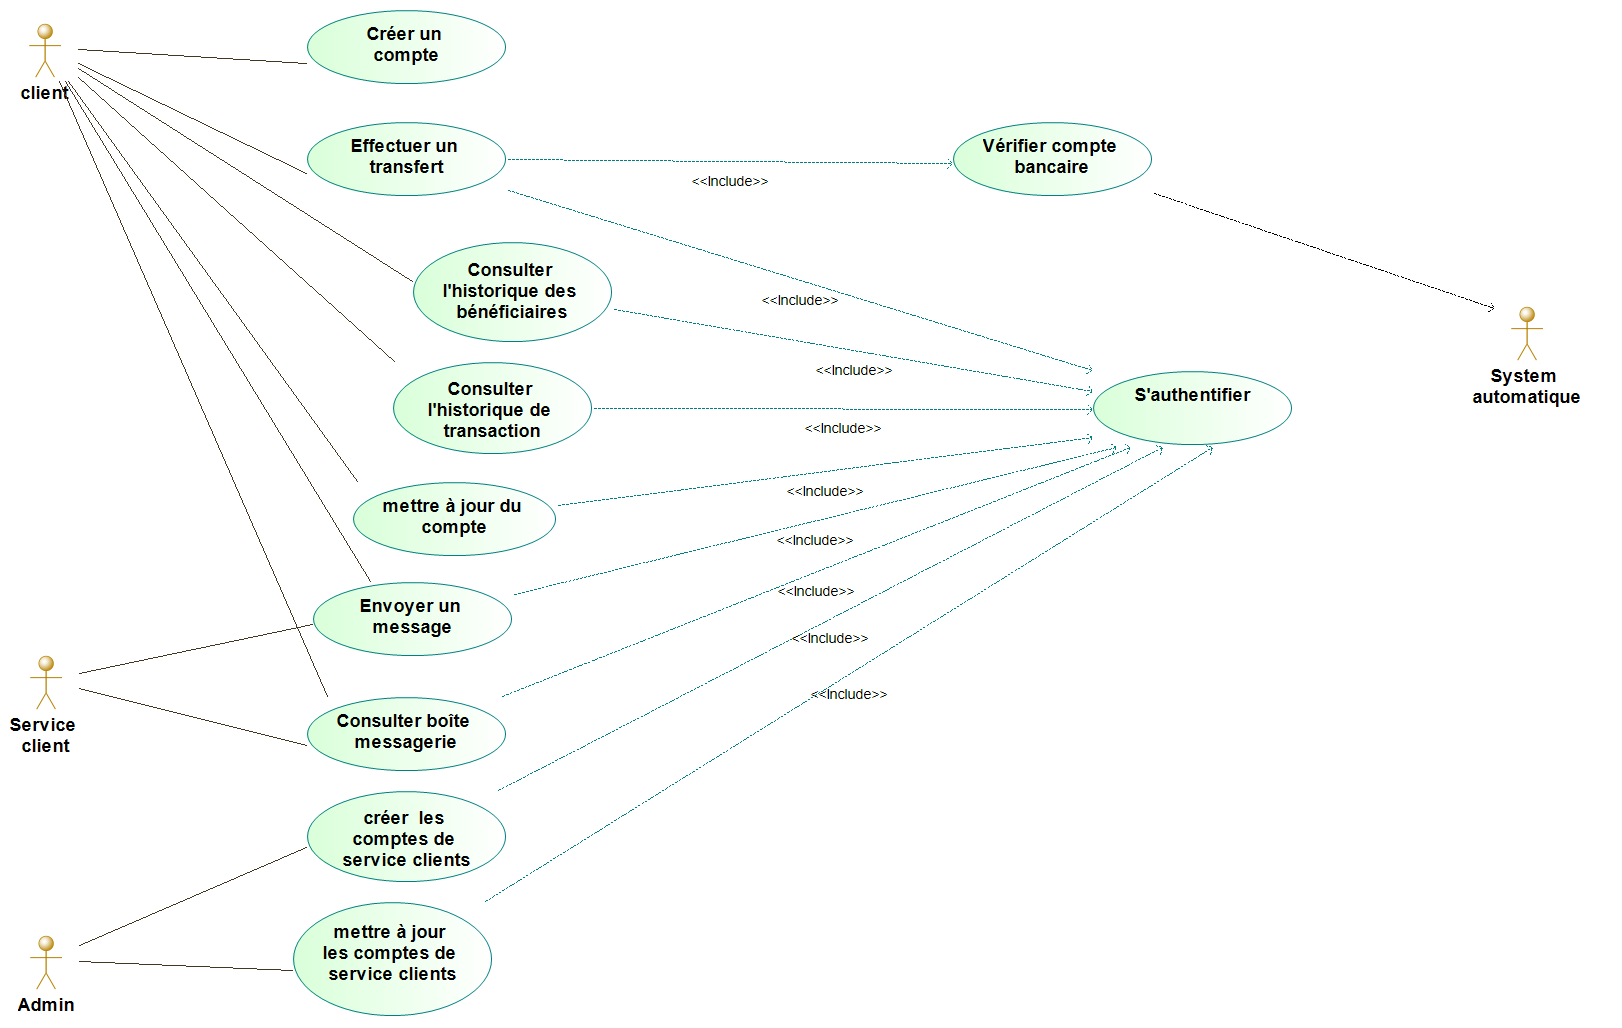
\includegraphics[width=18cm, height=12cm]{./Template LaTeX/Images/use_case.png}
	\caption{Diagramme de cas d’utilisation.}
	\label{fig1:use_case}
\end{figure}
%\textbf{Description détaillée des cas d'utilisation :}
\begin{comment}

\begin{table}[h]
	\begin{tabular}{|m{5cm}|m{2cm}|m{10cm}|}
		\hline
		\textbf{Cas d’utilisation} & \textbf{Acteur} & \textbf{Description}\\
		\hline
		\textbf{Créer un compte }&Client&L'utilisateur se renseigne pour créer un compte au sein de Cadorim pour
		pouvoir accéder au fonctionnalités proposées .\\
		\hline
		\textbf{S’authentifier}&Client&L'utilisateur saisit son identifiant et son mot de passe pour
		accéder aux fonctionnalités.\\
		\hline
		\textbf{Effectuer un transfert}&Client&L'utilisateur saisi le numéro du bénéficiaire et le montant a transférer.
		Une page de vérification avec les informations saisies.
		Transfère le montant vers le bénéficiaire.\\
		\hline
		\textbf{Créer un compte}&Client&L'utilisateur se renseigne pour créer un compte au sein de mauripay pour
		pouvoir accéder au fonctionnalités proposées .\\
		\hline
		\textbf{Créer un compte}&Client&L'utilisateur se renseigne pour créer un compte au sein de mauripay pour
		pouvoir accéder au fonctionnalités proposées .\\
		\hline
		\textbf{Créer un compte}&Client&L'utilisateur se renseigne pour créer un compte au sein de mauripay pour
		pouvoir accéder au fonctionnalités proposées .\\
		\hline
		
	
			
	\end{tabular}
	\caption{Description détaillée des cas d'utilisation}
	\label{4.1}
\end{table}
\end{comment}


	%\textbf{• Description détaillée des cas d'utilisation  :}
\begin{comment}
	
\begin{table}[h]
	\begin{tabular}{|m{4cm}|m{13.5cm}|}
		\hline
		\textbf{Cas d’utilisation}   \textbf{Description}\\
		\hline
		Créer un compte&L'utilisateur se renseigne pour créer un compte au sein de Cadorim pour
		pouvoir accéder au fonctionnalités proposées .\\
		\hline
		S’authentifier&L'utilisateur saisit son identifiant et son mot de passe pour
		accéder aux fonctionnalités.\\
		\hline
		Effectuer un transfert&L'utilisateur saisi le montant a transférer et les informations de  bénéficiaire.
		\newline Une page de vérification avec les informations saisies.
		\newline Transfère le montant vers le bénéficiaire.\\
		\hline
		Consulter l'historique des bénéficaires&L'utilisateur peut voire liste des bénéficaires \\
		\hline
		Consulter l'historique des transactions&L'utilisateur peut voire liste des transactions\\
		\hline
		mettre à jour du compte&L'utilisateur se renseigne pour créer un compte au sein de mauripay pour
		pouvoir accéder au fonctionnalités proposées .\\
		\hline
		Envoyer un message&L'utilisateur se renseigne pour créer un compte au sein de mauripay pour
		pouvoir accéder au fonctionnalités proposées .\\
		\hline
			Consulter boite \newline messagerie&L'utilisateur se renseigne pour créer un compte au sein de mauripay pour
		pouvoir accéder au fonctionnalités proposées .\\
		\hline
		
		
		
	\end{tabular}
	\caption{Description détaillée des cas d'utilisation d'acteur client}
	\label{4.1}
\end{table}
	content...
\end{comment}
%\newpage
\textbf{\hspace*{-1cm}• Description détaillée des cas d'utilisation  :\newline}
\begin{table}[h]
	\hspace*{-2cm}
	\begin{tabular}{|m{19.8cm}|}
		\hline
		\begin{center}
		 \textbf{Cas d’utilisation : Créer un compte, S’authentifier et Créer les comptes de service clients }
		\end{center}
		\\
		[-4ex] 
		\hline
			\begin{tabular}{m{3cm}|m{14cm}}
			
				\centering 	\textbf{Titre} & Créer un compte , S’authentifier , Créer les comptes de service clients
				\\
				[0ex] 
			\end{tabular}
		\\
		
		\hline
			\begin{tabular}{m{3cm}|m{14cm}}
			
			\centering 	\textbf{But} & Créer un compte pour accéder aux fonctionnalités de l’application 	\\
			[0ex] 
			
		\end{tabular}
		\\
		\hline
			\begin{tabular}{m{3cm}|m{15.5cm}}
			
			\centering 	\textbf{Résumé} & L'utilisateur doit remplir un formulaire d’inscription et identifier électroniquement leur document comme des pièces d’identité (carte d’identité, passeport ) à partir de leur caméra du téléphone puis valide son action.\newline Le système effectue une vérification puis une mise à jour de la base de données.
			\\
			[0ex] 
		\end{tabular}
		\\
		
		\hline
			\begin{tabular}{m{3cm}|m{14cm}}
			
			\centering 	\textbf{Acteurs } & Client,Admin \\[0ex]
			
		\end{tabular}
		\\
		 
		\hline
		\begin{center}
			\textbf{Descriptions des enchainements}
		\end{center}
		\\
		[-4ex] 
		\hline	
			\begin{tabular}{m{9.3cm}|m{9.3cm}}
			
			\begin{center}
				\textbf{Pré condition}
			\end{center}
		 		& 
		 	\begin{center}
				\textbf{Post condition}
			\end{center}
			\\[-4ex]
		\end{tabular}
		\\
		
		\hline
			\begin{tabular}{m{9.3cm}|m{9.3cm}}
			L'utilisateur doit accéder au système
			& 
			L'utilisateur inscrit
		\end{tabular}
		\\
		\hline
			\begin{center}
			\textbf{Scenario nominal}
			\end{center}
		\\
		[-4ex]
		\hline
		\begin{enumerate}
			\item [1.] L’utilisateur demande la page d’inscription en cliquant sur «S'INSCRIRE»
			\item [2.] Le système lui envoie la page d’inscription
			\item [3.] L’utilisateur rempli le formulaire et scanne leur document puis appuie sur S'INSCRIRE
			\item [4.] Le système effectue les validations et l’enregistrement dans la base de données
			\item [5.] L’utilisateur est redirigé vers la page d’authentification et renseigne ses identifiants en cas d'acteur client 
		\end{enumerate}
		\\
		[-4ex]
		\hline	
			\begin{center}
			\textbf{Enchainement d’échec }
		\end{center}
		\\ 
		[-4ex]
		\hline
		\begin{tabular}{m{17.5cm}}
			\begin{enumerate}
				\item [6.] Le compte existe déjà ou les données saisies sont incorrectes
				\item [7.] Il n’y a pas de connexion internet
			\end{enumerate}
			\\[-4ex]
		\end{tabular}
		\\
		\hline	
		
	\end{tabular}
	\centering \caption{Description détaillée des cas d'utilisation : Créer un compte  et S’authentifier}
	\label{4.1}
\end{table}
\newpage

\begin{table}[h]
	\hspace*{-2cm}
	\vspace*{-2cm}
	\begin{tabular}{|m{19.8cm}|}
		\hline
		\begin{center}
			\textbf{Cas d’utilisation : Effectuer transfert}
		\end{center}
		\\
		[-4ex] 
		\hline
		\begin{tabular}{m{3cm}|m{14cm}}
			
			\centering 	\textbf{Titre} & Effectuer transfert
			\\
			[0ex] 
		\end{tabular}
		\\
		
		\hline
		\begin{tabular}{m{3cm}|m{14cm}}
			
			\centering 	\textbf{But} & Envoyer de l’argent à un bénéficiaire	\\
			[0ex] 
			
		\end{tabular}
		\\
		\hline
		\begin{tabular}{m{3cm}|m{15.5cm}}
			
			\centering 	\textbf{Résumé} & L’utilisateur saisit les informations du bénéficiaire et le montant de la transaction et valide. Le système envoyait les informations de la carte bancaire au  fournisseur de paiement  avant de finaliser l’opération.
			\\
			[0ex] 
		\end{tabular}
		\\
		
		\hline
		\begin{tabular}{m{3cm}|m{14cm}}
			
			\centering 	\textbf{Acteurs } & Client \\[0ex]
			
		\end{tabular}
		\\
		
		\hline
		\begin{center}
			\textbf{Descriptions des enchainements}
		\end{center}
		\\
		[-4ex] 
		\hline	
		\begin{tabular}{m{9.3cm}|m{9.3cm}}
			
			\begin{center}
				\textbf{Pré condition}
			\end{center}
			& 
			\begin{center}
				\textbf{Post condition}
			\end{center}
			\\[-4ex]
		\end{tabular}
		\\
		
		\hline
		\begin{tabular}{m{9.3cm}|m{9.3cm}}
			- L’utilisateur doit se connecter \newline
			- L’utilisateur doit utiliser une carte bancaire valide & 
			- Le transfert est effectué \newline
			- Afficher  l'historique des transactions
			\\[0ex]
		\end{tabular}
		\\
		\hline
		\begin{center}
			\textbf{Scenario nominal}
		\end{center}
		\\
		[-4ex]
		\hline
		\begin{enumerate}
			\item [1.] L’utilisateur accède au formulaire de transfert en saisit le montant puis  cliquant sur « Envoyer »
			\item [2.] Le système lui demande de saisir les informations de transfert
			\item [3.] L’utilisateur rempli le formulaire appuie sur le bouton « Valider »
			\item [4.] Le système débiter le compte de cadorim et crédité le compte de bénéficiaire
			\item [5.] Le système lui affiche la page de l'historique des transactions
		\end{enumerate}
		\\
		[-4ex]
		\hline	
		\begin{center}
			\textbf{Enchainement d’échec }
		\end{center}
		\\ 
		[-4ex]
		\hline
		\begin{tabular}{m{17.5cm}}
			\begin{enumerate}
				\item [6.] La carte bancaire invalide ou le solde est insuffisant
				\item [7.] La saisie de données n’est pas correcte
				\item [8.] La connexion n’est pas bonne pour effectuer et suivre un transfert
			\end{enumerate}
			\\[-4ex]
		\end{tabular}
		\\
		\hline	
		
	\end{tabular}
	\vspace*{1.5cm}
	\centering \caption{Description détaillée des cas d'utilisation : Effectuer transfert}
	\label{4.1}
\end{table}

\newpage

\begin{table}[h]
	\hspace*{-2cm}
	\vspace*{-2.5cm}
	\begin{tabular}{|m{19.8cm}|}
		\hline
		\begin{center}
			\textbf{Cas d’utilisation : Consulter l'historique des bénéficiaires et l'historique de transaction}
		\end{center}
		\\
		[-4ex] 
		\hline
		\begin{tabular}{m{3cm}|m{14cm}}
			
			\centering 	\textbf{Titre} & Consulter l'historique des bénéficiaires,Consulter l'historique de transaction
			\\
			[0ex] 
		\end{tabular}
		\\
		
		\hline
		\begin{tabular}{m{3cm}|m{14cm}}
			
			\centering 	\textbf{But} & Consultations de l'historique\\
			[0ex] 
			
		\end{tabular}
		\\
		\hline
		\begin{tabular}{m{3cm}|m{15.5cm}}
			
			\centering 	\textbf{Résumé} & L'utilisateur voit les renseignements sur le bénéficiaire et l'opération de transaction.
			\\
			[0ex] 
		\end{tabular}
		\\
		
		\hline
		\begin{tabular}{m{3cm}|m{14cm}}
			
			\centering 	\textbf{Acteurs } & Client \\[0ex]
			
		\end{tabular}
		\\
		
		\hline
		\begin{center}
			\textbf{Descriptions des enchainements}
		\end{center}
		\\
		[-4ex] 
		\hline	
		\begin{tabular}{m{9.3cm}|m{9.3cm}}
			
			\begin{center}
				\textbf{Pré condition}
			\end{center}
			& 
			\begin{center}
				\textbf{Post condition}
			\end{center}
			\\[-4ex]
		\end{tabular}
		\\
		
		\hline
		\begin{tabular}{m{9.3cm}|m{9.3cm}}
			- L’utilisateur doit se connecter \newline
			 & 
			- Afficher  l'historique des transactions ou des  \newline bénéficiaires
			\\[0ex]
		\end{tabular}
		\\
		\hline
		\begin{center}
			\textbf{Scenario nominal}
		\end{center}
		\\
		[-4ex]
		\hline
		\begin{enumerate}
			\item [1.] L’utilisateur accède a l'historique des transactions ou des bénéficiaires en cliquant sur « Transferts » ou « Benef »
			\item [2.] Le système lui affiche la page de l'historique
		\end{enumerate}
		\\
		[-4ex]
		\hline	
		\begin{center}
			\textbf{Enchainement d’échec }
		\end{center}
		\\ 
		[-4ex]
		\hline
		\begin{tabular}{m{17.5cm}}
			\begin{enumerate}
				\item [3.] Il n’y a pas de connexion internet
				
			\end{enumerate}
			\\[-4ex]
		\end{tabular}
		\\
		\hline	
		
	\end{tabular}
	\vspace*{2cm}
	\centering \caption{Description détaillée des cas d'utilisation : Consulter l'historiques(des transactions ou des bénéficiaires)}
	\label{4.1}
\end{table}

\newpage

\begin{table}[h]
	\hspace*{-2cm}
	\vspace*{-2cm}
	\begin{tabular}{|m{19.8cm}|}
		\hline
		\begin{center}
			\textbf{Cas d’utilisation : Consulter boite messagerie}
		\end{center}
		\\
		[-4ex] 
		\hline
		\begin{tabular}{m{3cm}|m{14cm}}
			
			\centering 	\textbf{Titre} & Consulter boite messagerie
			\\
			[0ex] 
		\end{tabular}
		\\
		
		\hline
		\begin{tabular}{m{3cm}|m{14cm}}
			
			\centering 	\textbf{But} & Consulter boite messagerie\\
			[0ex] 
			
		\end{tabular}
		\\
		\hline
		\begin{tabular}{m{3cm}|m{15.5cm}}
			
			\centering 	\textbf{Résumé} &L'utilisateur voit l'historique des  messages et les messages reçus.
			\\
			[0ex] 
		\end{tabular}
		\\
		
		\hline
		\begin{tabular}{m{3cm}|m{14cm}}
			
			\centering 	\textbf{Acteurs } & Client, Srvice client \\[0ex]
			
		\end{tabular}
		\\
		
		\hline
		\begin{center}
			\textbf{Descriptions des enchainements}
		\end{center}
		\\
		[-4ex] 
		\hline	
		\begin{tabular}{m{9.3cm}|m{9.3cm}}
			
			\begin{center}
				\textbf{Pré condition}
			\end{center}
			& 
			\begin{center}
				\textbf{Post condition}
			\end{center}
			\\[-4ex]
		\end{tabular}
		\\
		
		\hline
		\begin{tabular}{m{9.3cm}|m{9.3cm}}
			- L’utilisateur doit se connecter \newline
			& 
			- Afficher  l'historique des  messages et les messages reçus
			\\[0ex]
		\end{tabular}
		\\
		\hline
		\begin{center}
			\textbf{Scenario nominal}
		\end{center}
		\\
		[-4ex]
		\hline
		\begin{enumerate}
			\item [1.] L’utilisateur accède à la boîte messagerie
			\item [2.] Le système lui affiche la page des messageries
		\end{enumerate}
		\\
		[-4ex]
		\hline	
		\begin{center}
			\textbf{Enchainement d’échec }
		\end{center}
		\\ 
		[-4ex]
		\hline
		\begin{tabular}{m{17.5cm}}
			\begin{enumerate}
				\item [3.] Il n’y a pas de connexion internet
				
			\end{enumerate}
			\\[-4ex]
		\end{tabular}
		\\
		\hline	
		
	\end{tabular}
	\vspace*{1.5cm}
	\centering \caption{Description détaillée des cas d'utilisation : Consulter boite messagerie}
	\label{4.1}
\end{table}


\newpage

\begin{table}[h]
	\hspace*{-2cm}
	\vspace*{-2cm}
	\begin{tabular}{|m{19.8cm}|}
		\hline
		\begin{center}
			\textbf{Cas d’utilisation : Envoyer un message}
		\end{center}
		\\
		[-4ex] 
		\hline
		\begin{tabular}{m{3cm}|m{14cm}}
			
			\centering 	\textbf{Titre} & Envoyer un message
			\\
			[0ex] 
		\end{tabular}
		\\
		
		\hline
		\begin{tabular}{m{3cm}|m{14cm}}
			
			\centering 	\textbf{But} & Envoyer un message\\
			[0ex] 
			
		\end{tabular}
		\\
		\hline
		\begin{tabular}{m{3cm}|m{15.5cm}}
			
			\centering 	\textbf{Résumé} &L'utilisateur peut envoyer un message où répond à un message
			\\
			[0ex] 
		\end{tabular}
		\\
		
		\hline
		\begin{tabular}{m{3cm}|m{14cm}}
			
			\centering 	\textbf{Acteurs } & Client, Srvice client \\[0ex]
			
		\end{tabular}
		\\
		
		\hline
		\begin{center}
			\textbf{Descriptions des enchainements}
		\end{center}
		\\
		[-4ex] 
		\hline	
		\begin{tabular}{m{9.3cm}|m{9.3cm}}
			
			\begin{center}
				\textbf{Pré condition}
			\end{center}
			& 
			\begin{center}
				\textbf{Post condition}
			\end{center}
			\\[-4ex]
		\end{tabular}
		\\
		
		\hline
		\begin{tabular}{m{9.3cm}|m{9.3cm}}
			- L’utilisateur doit se connecter \newline
			& 
			\centering - Le message est envoyé
			\\[0ex]
		\end{tabular}
		\\
		\hline
		\begin{center}
			\textbf{Scenario nominal}
		\end{center}
		\\
		[-4ex]
		\hline
		\begin{enumerate}
			\item [1.] L’utilisateur demande le formulaire d’envoi de message
			\item [2.] Le système lui affiche la page des discussions
		\end{enumerate}
		\\
		[-4ex]
		\hline	
		\begin{center}
			\textbf{Enchainement d’échec }
		\end{center}
		\\ 
		[-4ex]
		\hline
		\begin{tabular}{m{17.5cm}}
			\begin{enumerate}
				\item [3.] Il n’y a pas de connexion internet
				
			\end{enumerate}
			\\[-4ex]
		\end{tabular}
		\\
		\hline	
		
	\end{tabular}
	\vspace*{1.5cm}
	\centering \caption{Description détaillée des cas d'utilisation : Envoyer un message}
	\label{4.1}
\end{table}
\begin{comment}

	\item[•]  \textbf{Description détaillée des cas d'utilisation d'acteur service client :}
\begin{table}[h]
	\begin{tabular}{|m{4cm}|m{13.5cm}|}
		\hline
		\textbf{Cas d’utilisation}  & \textbf{Description}\\
		\hline
		Enoyer un message&L'utilisateur se renseigne pour créer un compte au sein de Cadorim pour
		pouvoir accéder au fonctionnalités proposées .\\
		\hline
		S’authentifier&L'utilisateur saisit son identifiant et son mot de passe pour
		accéder aux fonctionnalités.\\
		\hline
			Consulter boite \newline messagerie&L'utilisateur saisit son identifiant et son mot de passe pour
		accéder aux fonctionnalités.\\
		\hline
	\end{tabular}
	\caption{Description détaillée des cas d'utilisation d'acteur service client}
	\label{4.1}
\end{table}

	\item[•]  \textbf{Description détaillée des cas d'utilisation d'acteur admin :}
\begin{table}[h]
	\begin{tabular}{|m{4cm}|m{13.5cm}|}
		\hline
		\textbf{Cas d’utilisation}  & \textbf{Description}\\
		\hline
		Créer les comptes de service clients&L'utilisateur se renseigne pour créer un compte au sein de Cadorim pour
		pouvoir accéder au fonctionnalités proposées .\\
		\hline
		S’authentifier&L'utilisateur saisit son identifiant et son mot de passe pour
		accéder aux fonctionnalités.\\
		\hline
		Mettre à jour les comptes de service clients&L'utilisateur saisit son identifiant et son mot de passe pour
		accéder aux fonctionnalités.\\
		\hline
	\end{tabular}
	\caption{Description détaillée des cas d'utilisation d'acteur admin}
	\label{4.1}
\end{table}
\item[•]  \textbf{Description détaillée des cas d'utilisation d'acteur system :}
\begin{table}[h]
	\begin{tabular}{|m{4cm}|m{13.5cm}|}
		\hline
		\textbf{Cas d’utilisation}  & \textbf{Description}\\
		\hline
		 Vérifier compte \newline bancaire&L'utilisateur se renseigne pour créer un compte au sein de Cadorim pour
		pouvoir accéder au fonctionnalités proposées .\\
		\hline
	\end{tabular}
	\caption{Description détaillée des cas d'utilisation d'acteur secondaire system}
	\label{4.1}
\end{table}
	content...
\end{comment}


\subsection{Diagramme d’activité}
Cette section a pour objectif de mettre en surbrillance le processus quelques fonctionnalités de
l’application pour voir les détailles. J’ai choisi trois cas d’utilisation, à savoir, la création d’un compte,la transfert d'argent et l'authentification.
\newpage
\subsubsection{Création de compte}
Le diagramme d’activité qu’illustre la figure~\ref{activiteCompte} décrit le cas d’utilisation « Créer un compte ».
\begin{figure}[h!]
	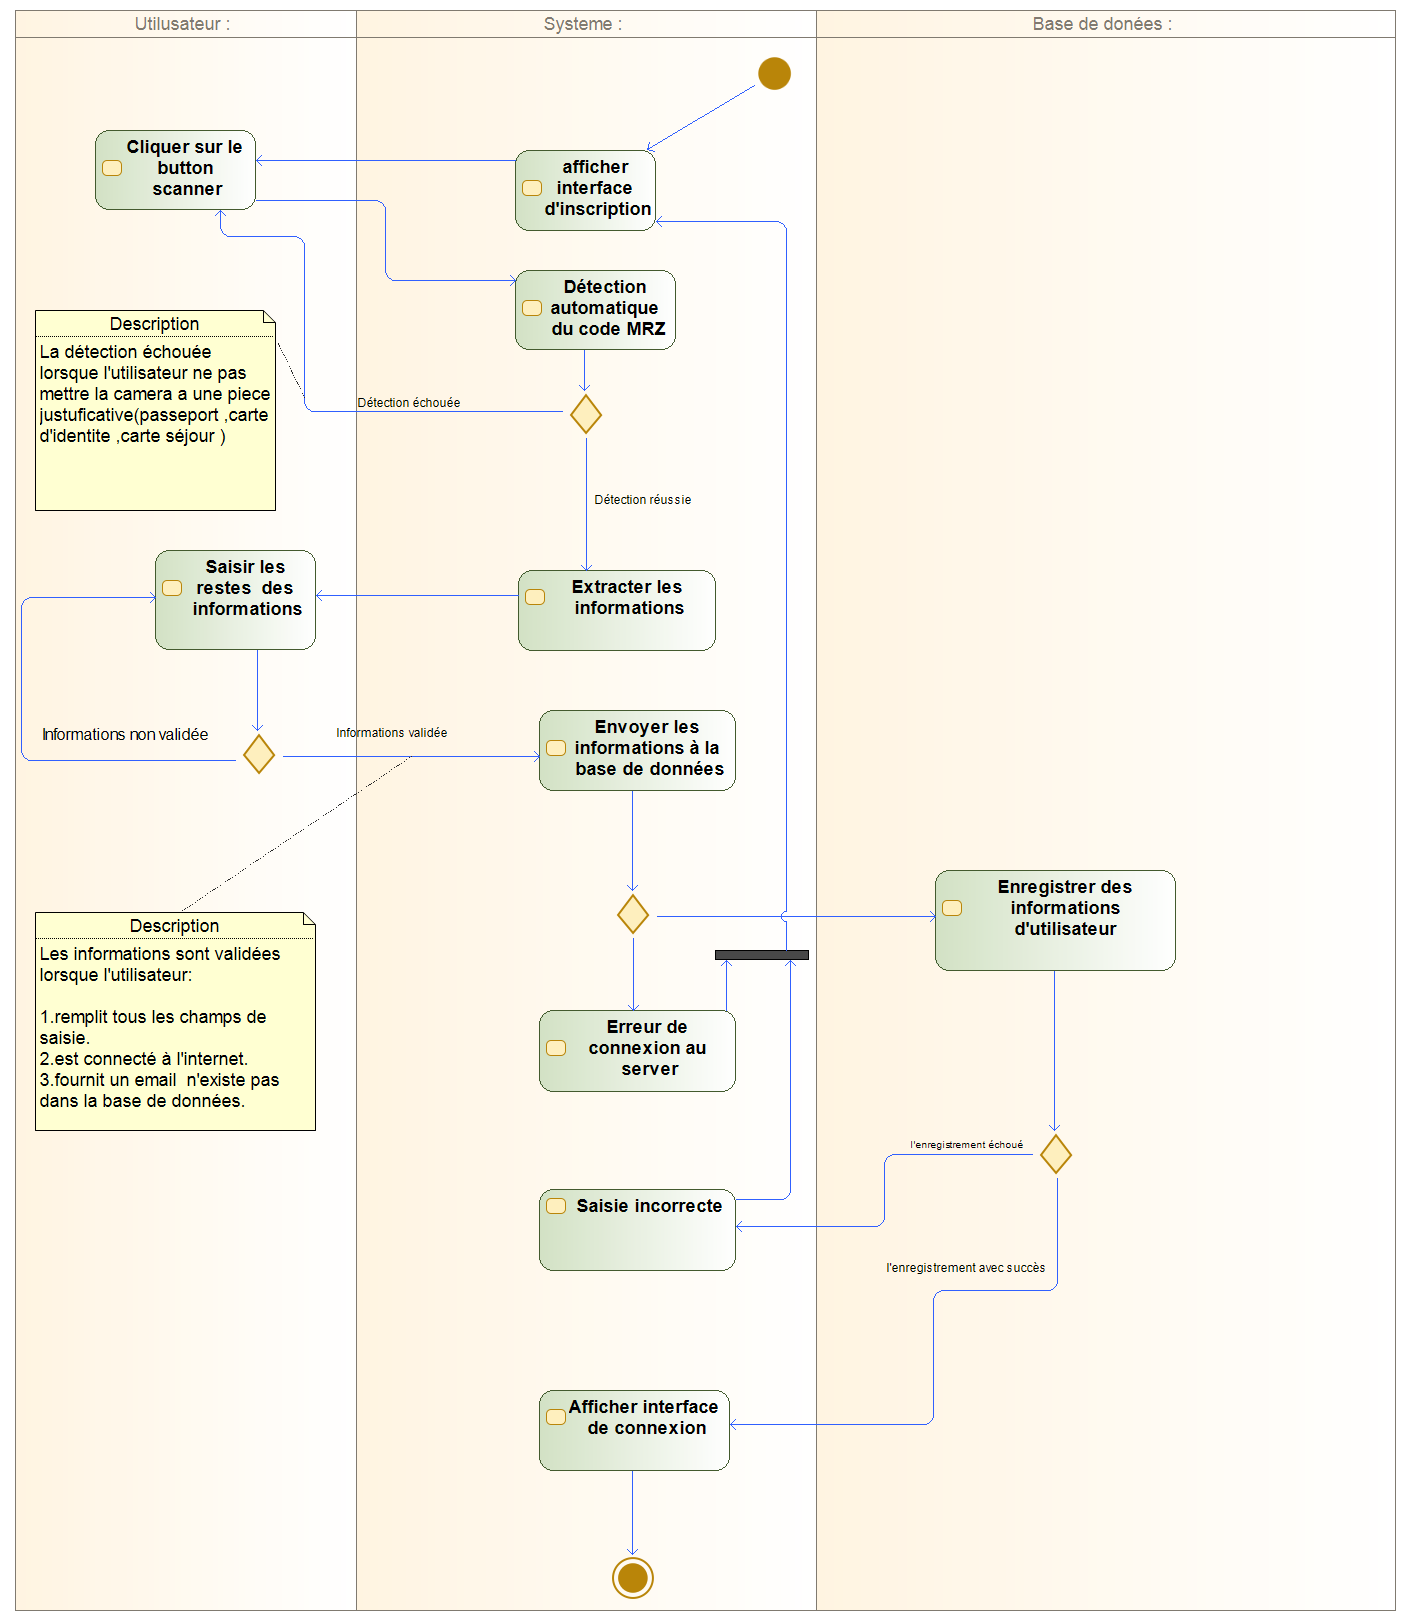
\includegraphics[width=18cm, height=19cm]{./Template LaTeX/Images/ins_act.png}
\caption{Diagramme d’activité : Création de compte}
\label{activiteCompte}

\end{figure}

\subsubsection{Transfert d'argent}
Le diagramme d’activité qu’illustre la figure~\ref{activiteTr} décrit les différentes actions ou enchainements
effectués lors d’une opération de transfert d’argent.
\begin{figure}[h!]
	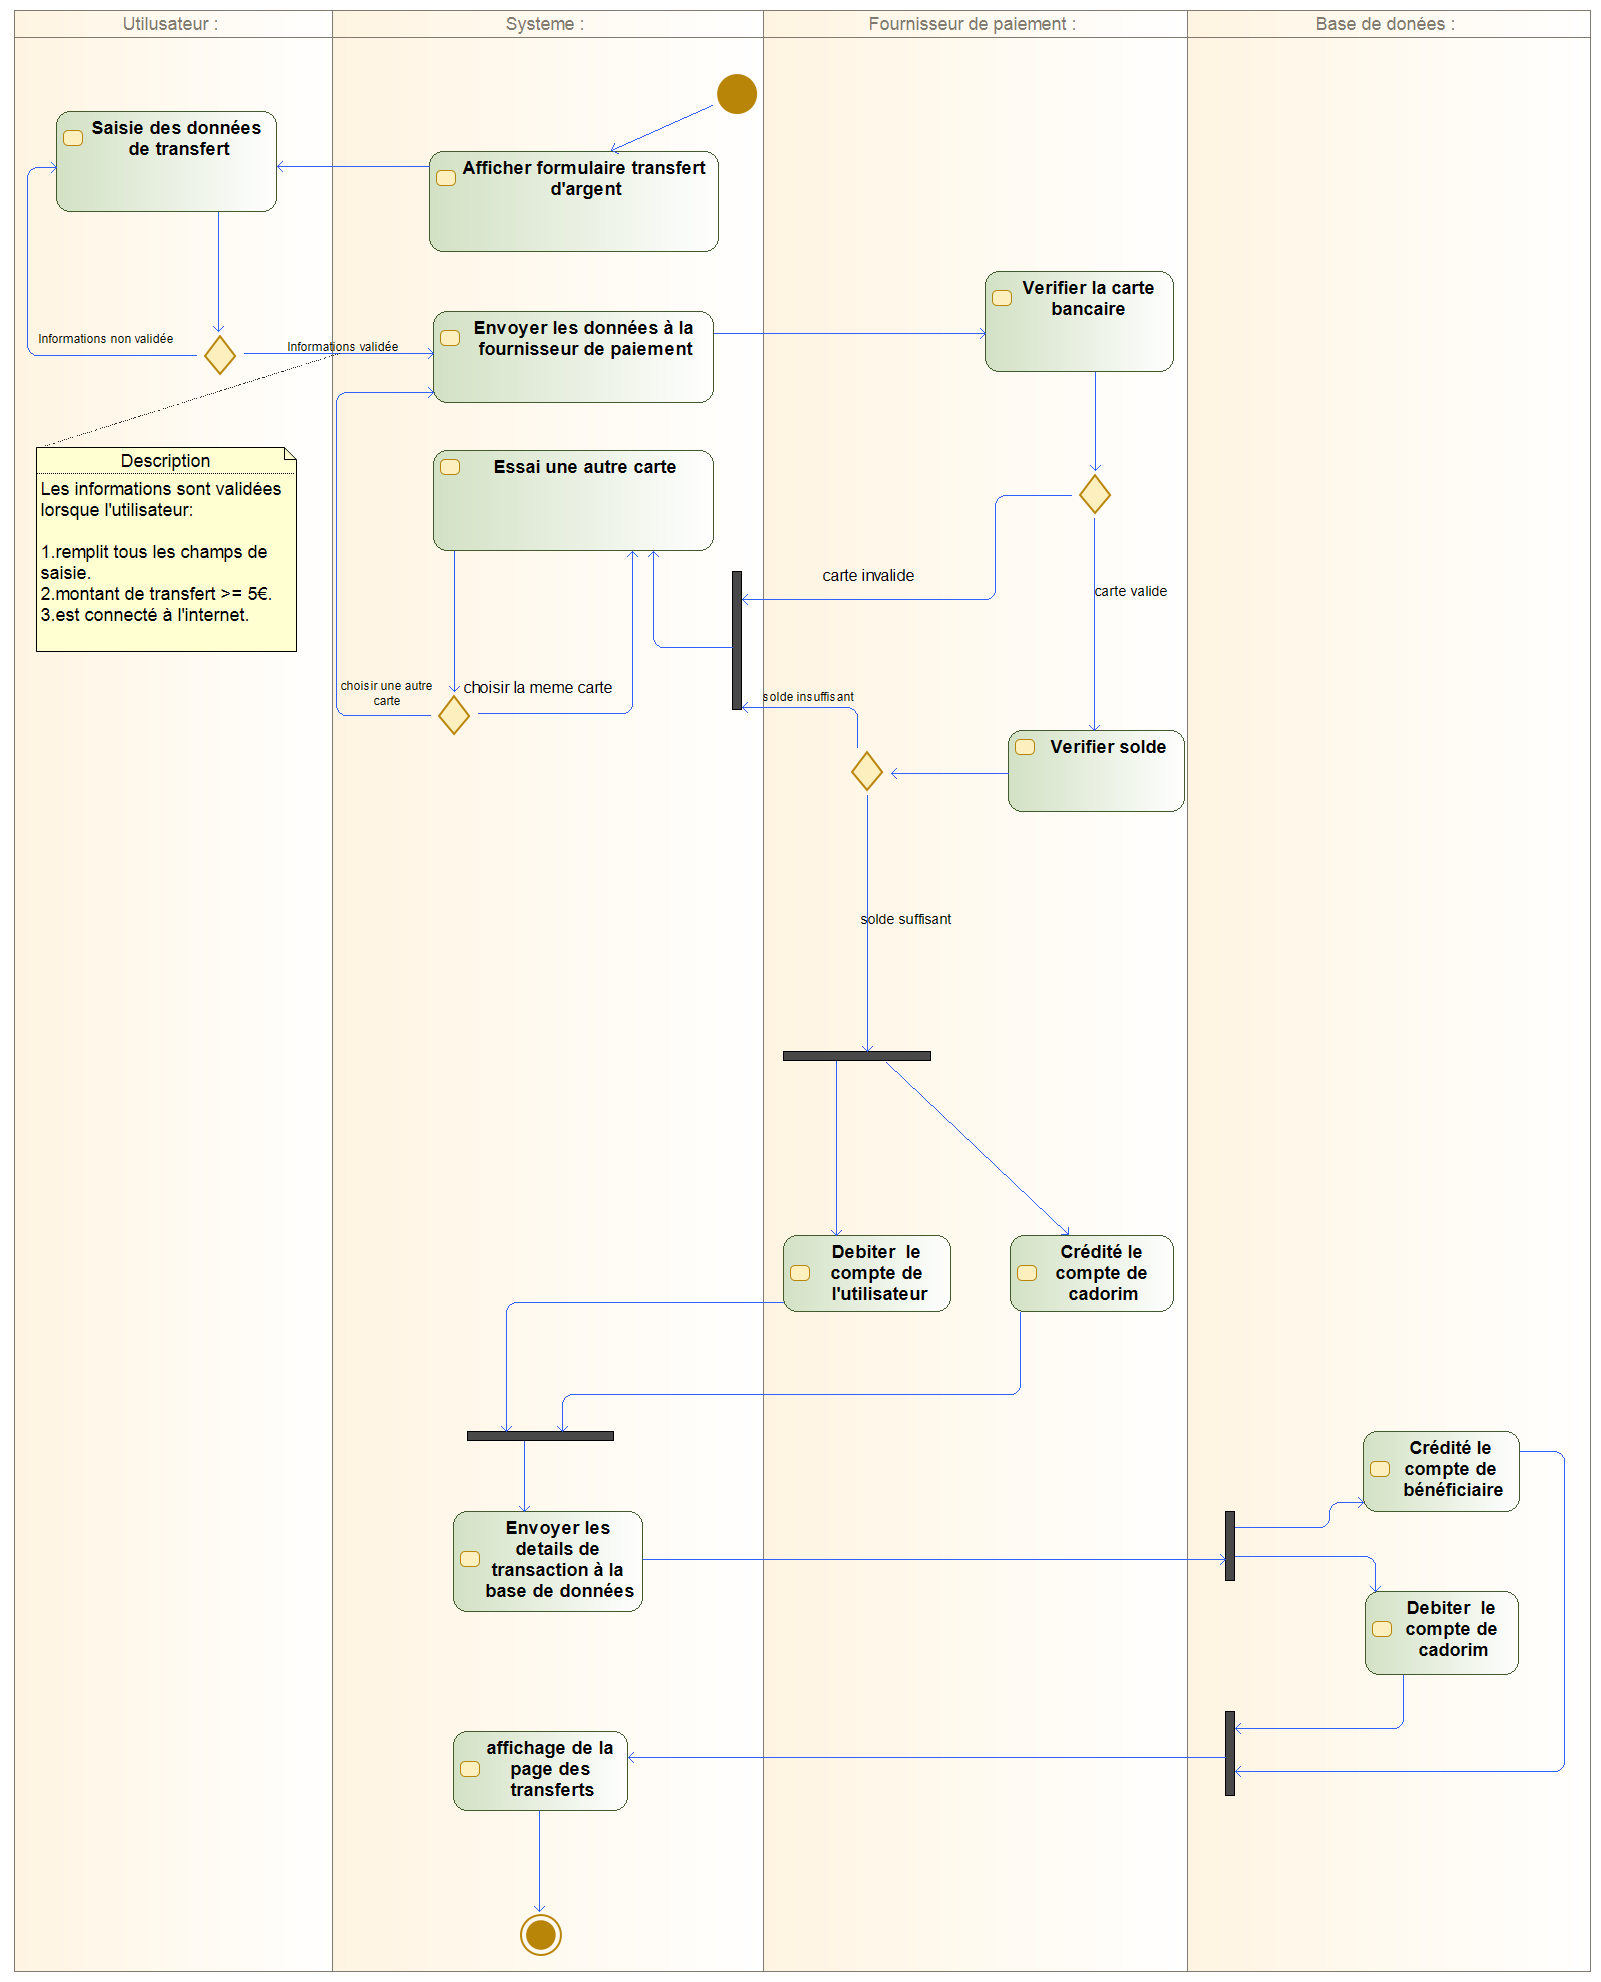
\includegraphics[width=18cm, height=20cm]{./Template LaTeX/Images/trans_act.png}
	\caption{Diagramme d'activité : Transfert d'argent}
	\label{activiteTr}
\end{figure}

\subsubsection{Authentification}
Le diagramme d’activité qu’illustre la figure~\ref{activiteAuth} décrit le cas d’utilisation « Authentification ».
\begin{figure}[h!]
	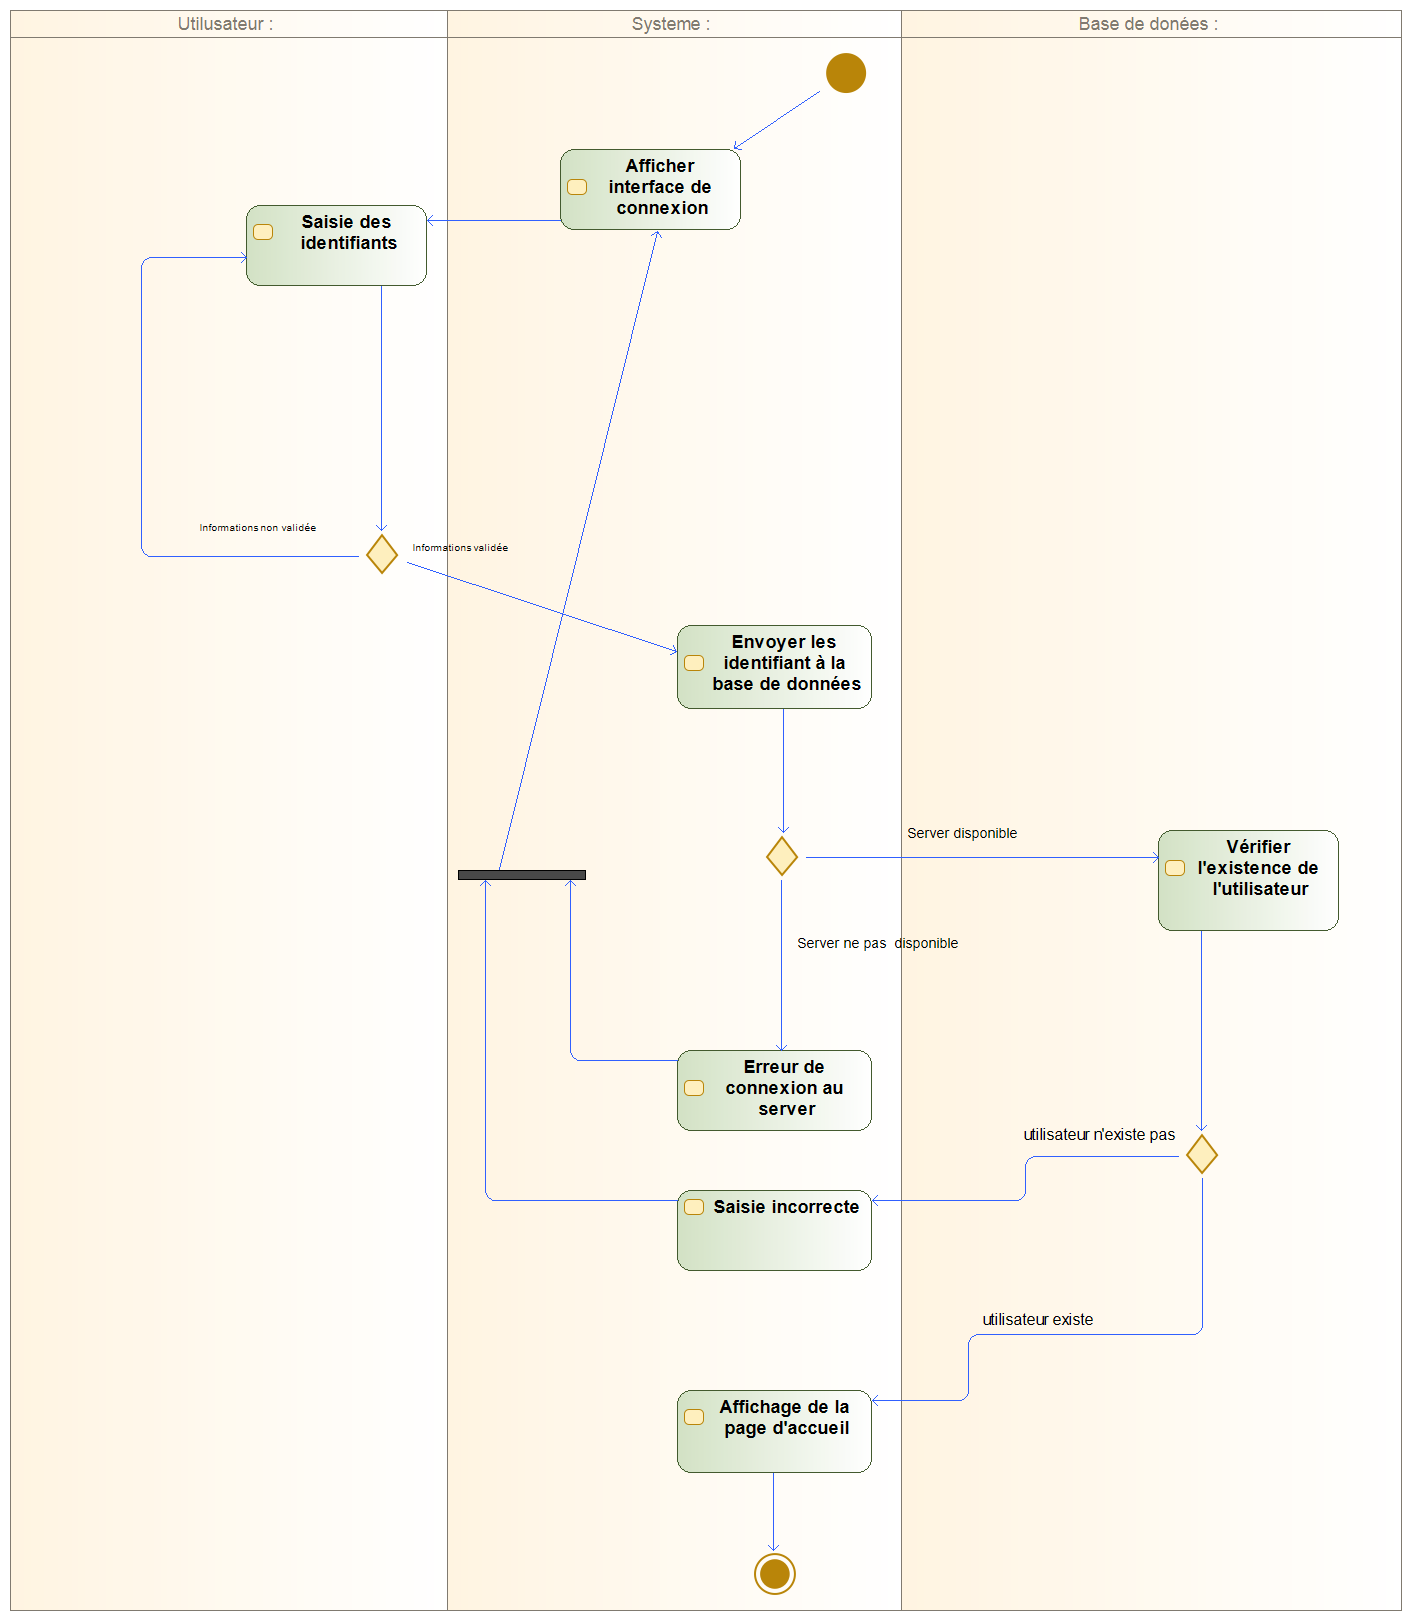
\includegraphics[width=18cm, height=20cm]{./Template LaTeX/Images/auth_act.png}
	\caption{Diagramme d'activité : Authentification}
	\label{activiteAuth}
\end{figure}


%\section{Modélisation de la base de données}
%\subsection{Diagramme de séquence}
%\newpage

\subsection{Diagramme de classe}
Afin de bien détailler l’architecture de la base de données, nous avons conçu le diagramme de
classe représenté dans la figure~\ref{fig4:class}.
\begin{figure}[h!]
	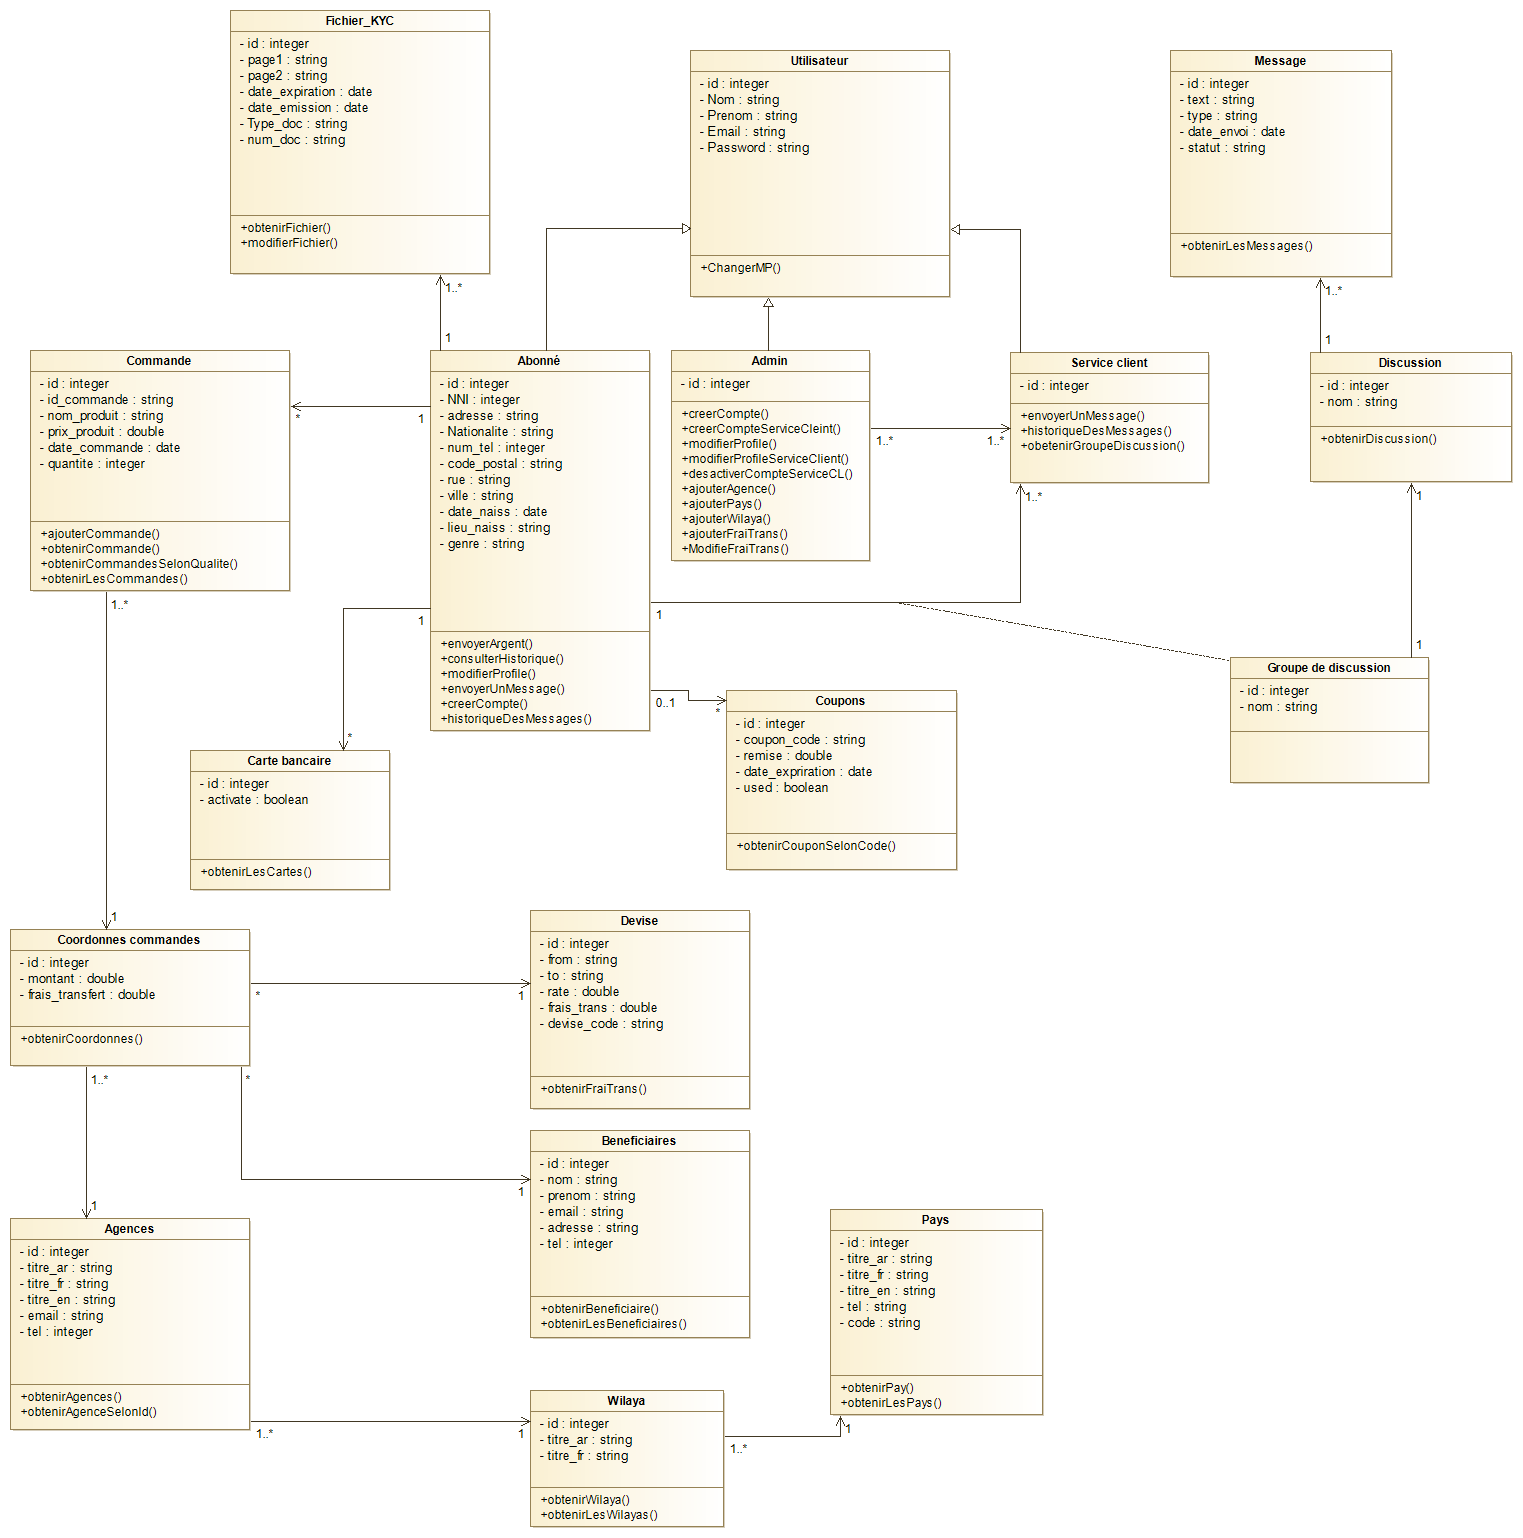
\includegraphics[width=18cm, height=20cm]{./Template LaTeX/Images/Diagramme_de_classe_V3.png}
	\caption{Diagramme de classe}
	\label{fig4:class}
\end{figure}
\newpage
\hspace*{-2cm} Le tableau~\ref{fig4:classT} explique les différentes classes de la base de données.
\begin{table}[h]
	\hspace*{-2cm}
	%\vspace*{6cm}
	\begin{tabular}{|m{5cm}|m{14cm}|}
		\hline
			\textbf{Classe}& \textbf{Description}
		\\
		\hline
		Abonné&Informations de l'utilisateur
		\\
		\hline
		Fichier KYC&  Contient les informations du fichier (carte d'identité, passeport, titre de séjour, carte bancaire) de client
		\\
			\hline
		Commande& Informations concernant une commande
		\\
			\hline
		Coordonnes commandes& Détails de chaque commande
		\\
			\hline
		Agences& Informations sur les agences de cadorim
		\\
			\hline
		Carte bancaire& Gestion de carte bancaire\\
		\hline	
			Devise& Informations sur la devise selon le pays d'envoi et le pays reçoivent
		\\
		\hline
			Beneficiaires&Informations sur les Beneficiaires
		\\
		\hline	
			Wilaya&Informations sur les Wilayas
		\\
		\hline	
			Admin&Informations de l’Admin et ses privilèges
		\\
		\hline	
			Service client&Service client avec certains privilèges
		\\
		\hline	
			Coupons&Informations d’un coupon
		\\
		\hline	
			Groupe de discussion&Informations sur les groupes
		\\
		\hline	
			Discussion&Informations de discussion de chaque groupe
		\\
		\hline		
			Message&Contient les messages de chaque discussion
		\\
		\hline
			Pays&Informations sur les pays
		\\
		\hline		
	\end{tabular}
	%\vspace*{10cm}
	\centering \caption{Description de la base de données}
	\label{fig4:classT}
\end{table}

%%%%%%%%%%%%%%%%%%%%%%%%%%%%%%%%%%%%%%%%%%%%5 ICI %%%%%%%%%%%%%%%%%%%%%%%%%%%%%%%%%%%%%%%%555


	\chapter{Environnement de travail}
	\label{sec:EnvironnementDeTravail}
	L'objectif de ce chapitre consiste à expliciter tous les éléments relatifs à l'environnement logiciel sur lequel j'ai travaillé pour réaliser cette application. Il s'agit donc des logiciels, langages, frameworks, et motifs d'architecture auxquels j'ai fait recours tout au long du processus de mise en œuvre de ma solution.
	\section{Gestion du projet}
	Dans cette section, je présente la méthodologie de travail et le logiciel de gestion de projet que j'ai utilisé pour déclencher, organiser et gérer le travail sur ma solution.
	\subsection{Méthodologie de travail}
	C'est la manière de mener un processus de développement. Il s’agit d’une démarche, un ensemble d’étapes ou procédures à mettre en œuvre dans une logique méthodologique, accompagnés d’outils et de techniques. L'utilisation d'une méthode est incontournable dans l'entreprise de tout projet, particulièrement dans la réalisation de projets informatiques. Dans ce cas-ci, les méthodes utilisées sont des méthodes d'analyse et de conception qui ont pour but la formalisation des étapes préliminaires au développement de systèmes logiciels, en d'autres termes : analyse, modélisation et conception. \newline
	L'urgence de l'utilisation de ces méthodes trouve son explication dans un certain nombre de facteurs :
	\begin{enumerate}
		\item De nombreux échecs de projets informatiques dans le passé dus à un manque d'organisation, ou une non satisfaction des besoins ;
		\item La révolution de l'industrie logicielle engendrée par les échecs informatiques et qui introduit de nouveaux facteurs de validation de la qualité logicielle : le génie logiciel ;
		\item Les nombreuses exigences liées au coût, aux délais et à la complexité des projets informatiques.
	\end{enumerate}
	
	L'utilisation de méthodes de développement de logiciels permet ainsi l'élaboration de systèmes informatiques de manière fiable et viable tout en répondant à l'ensemble des exigences du client et du génie logiciel.
	\newline \newline
	Il existe plusieurs méthodes de développement informatique. L’on distingue deux approches : l’approche traditionnelle et l’approche agile. Les deux approches se distinguent essentiellement dans la manière de décomposer le projet. Les méthodes cartésiennes ou fonctionnelles ou encore traditionnelles se sont imposées les premières.
	\subsubsection{L'approche traditionnelle}
	Cette approche s’inspire directement de l’architecture des ordinateurs. Les méthodes traditionnelles prônent une démarche strictement planifiée avec une séquence d’activités bien définie. La succession des activités et le planning doivent être clairement respectés et aucun changement n’est permis. Il est attendu du client une spécification des besoins globale, détaillée, claire, précise et validée en entrée. Ainsi, tout doit être prévisible, du début du projet à la livraison du produit, d’où l’appellation de méthodes prédictives. \newline
	Selon le planning adopté, les méthodes cartésiennes proposent plusieurs modèles d’exécution des activités du projet :
	\begin{enumerate}
		\item Le \textbf{modèle en cascade} : dans ce modèle, le processus de développement est découpé séquentiellement et de façon linéaire selon les activités intrinsèques du cycle de vie du développement logiciel : l’analyse, la conception, le codage et les tests. Le plan de déroulement des phases (planification prédictive) est élaboré en tout début de processus. Le passage à une phase donnée n’est fait que si le résultat de la phase précédente a été validé et jugé satisfaisant par le client et les utilisateurs.
		\item Le \textbf{modèle en V} : Le cycle en V est à la base de tout développement logiciel, il en représente les activités intrinsèques. Il tient d'avantage compte de la réalité que le modèle en cascade, le processus de développement n’est pas réduit à un enchainement de tâches séquentielles. Le modèle en V permet d’anticiper sur les phases ultérieures de développement du produit en particulier les plans de test de qualifications et de performance.
	\end{enumerate}
	Parmi les méthodes traditionnelles, nous pouvons citer : SADT, CORIG, …
	\subsubsection{L'approche agile}
	Cette approche est définie par les concepts suivants : la simplicité, la légèreté, la souplesse, un lien fort avec le client. C’est dans cette optique que certains apparentent le développement agile aux notions de flexibilité, de rétroaction et d’adaptation au changement rapide et continu.
	\newline
	Une méthode agile est une approche itérative et incrémentale, qui est menée dans un esprit collaboratif avec juste ce qu’il faut de formalisme. Elle génère un produit de haute qualité tout en prenant en compte l’évolution des besoins des clients et en anticipant sur les risques. Il y’a continuellement des aller et retour avec le client. L’application logicielle est livrée par version incrémentale. Les versions successives sont aussi fiables que le livrable final en termes de tests et de validation. En quelque sorte le processus est déroulé comme un enchaînement de « mini-cascades ». A chaque nouvelle itération, l’ensemble de l’architecture et de la conception logicielle est reconsidéré, le code est retravaillé.
	\newline
	Les méthodes agiles aspirent donc à améliorer la réactivité et l’adaptabilité des sociétés de logiciels et constituent un moyen de survie dans un environnement instable en s’accompagnant des valeurs suivantes :
	\begin{enumerate}
		\item Les individus et les interactions plutôt que les processus et les outils;
		\item L’application fonctionnelle plutôt que la documentation compréhensive;
		\item La collaboration avec le client plutôt que la négociation des contrats;
		\item La réponse au changement plutôt que le suivi d’un plan.
		\newline
	\end{enumerate}
	L’agilité comprend plusieurs courants de pensée qui ont conduits à des méthodes différentes, reposant sur les mêmes concepts mais présentant des singularités. Les méthodes Scrum, Kanban, et XP (eXtreme Programming) sont des exemples de ces méthodes.
	\newline\newline
	
	\textbf{La méthode SCRUM}
	\newline
	\textbf{Scrum} est une méthode agile de gestion de projet qui permet de produire la plus grande valeur métier dans la durée la plus courte. Elle a pour objectif d’améliorer la cohésion de l’équipe et la rapidité du processus de développement. Le nom Scrum renvoie à une pratique généralement connue au rugby signifiant la « mêlée ». \newline
	Cette méthode qualifie un ensemble de rôles, d’instruments de gestion et de pratiques managériales favorisant un environnement basé sur la transparence, l’inspection, le suivi et l’adaptation. Le cycle de vie d’un projet Scrum peut être découpé en trois parties :
	\begin{enumerate}
		\item Phase d'\textbf{initiation ou démarrage} : il s’agit d’une phase linéaire où l’on définit le périmètre fonctionnel du système et la liste des fonctionnalités (\textbf{Backlog}) agencées par ordre de priorité, d’effort, de complexité et de risque. C’est aussi à ce niveau que l’architecture est définie.
		
		\item Phase de \textbf{développement} est un processus empirique : le projet est découpé en cycles itératifs d’une durée de deux semaines ou \textbf{sprints}. Chaque sprint regroupe une ou plusieurs fonctionnalités du Backlog. Tout au long de cette phase, le travail réalisé est mesuré et contrôlé et une amélioration constante du prototype est faite.
		
		\item Phase de \textbf{Clôtures} est une phase linéaire de gestion de la livraison du produit final.
	\end{enumerate}
	La figure \ref{Scrum} montre l’articulation générale de Scrum. \newline
	\begin{figure}[h]
		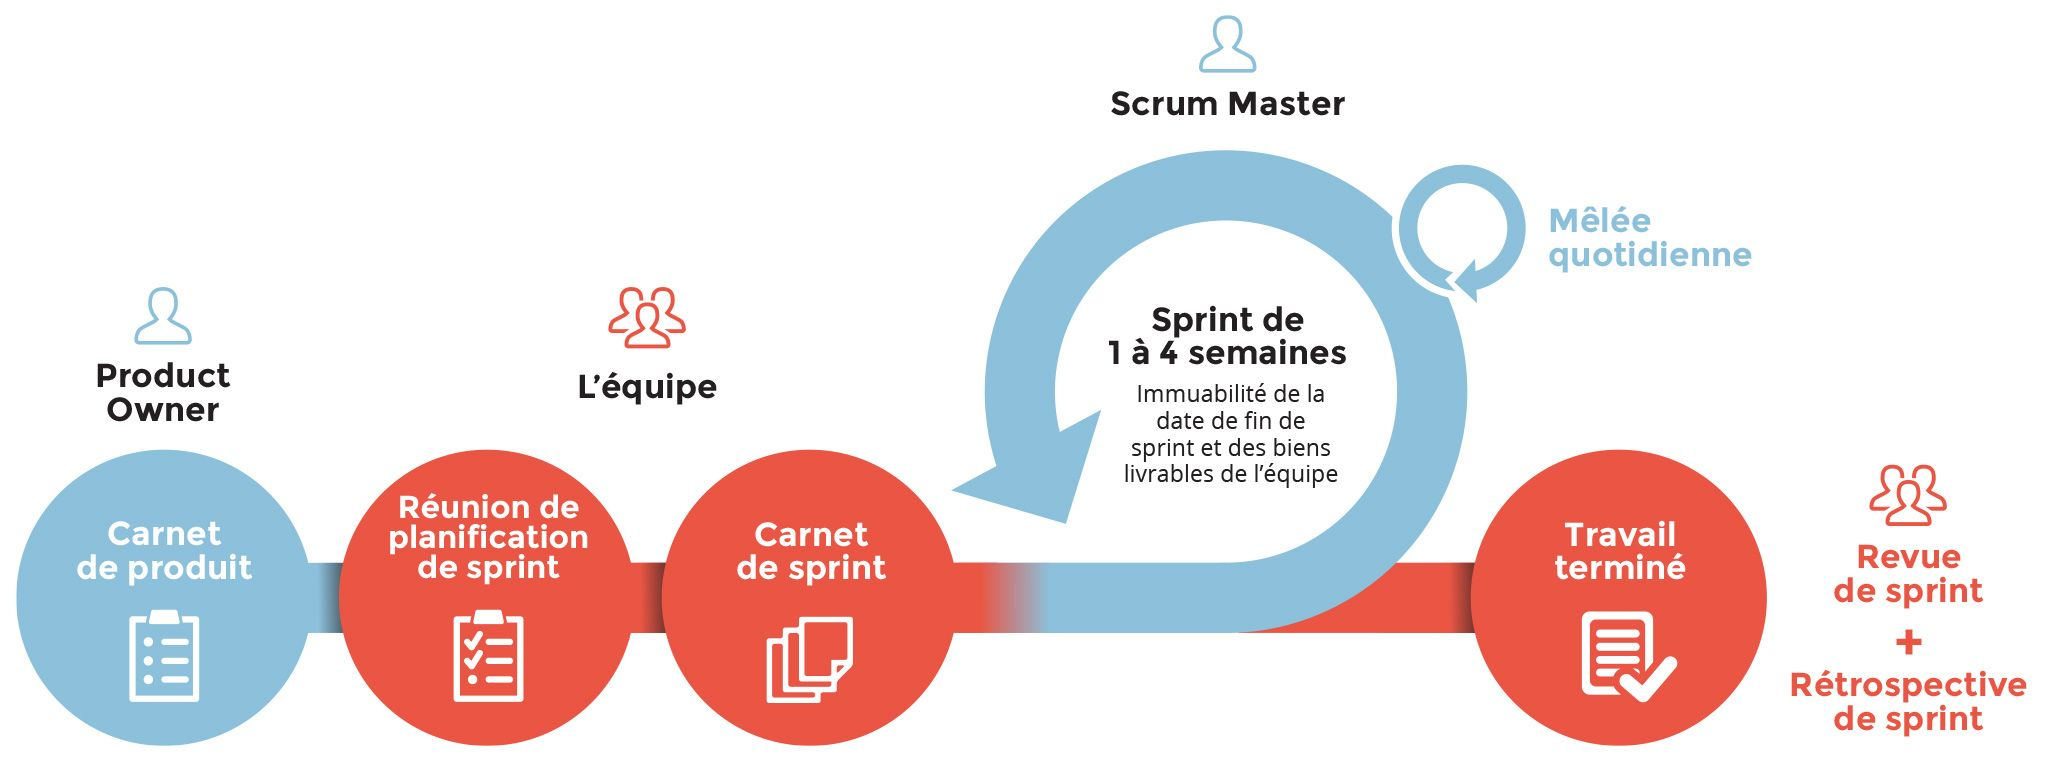
\includegraphics[width=15cm, height=5cm]{/home/mohamed/mes_fichier/CADORIM/LaTeX/pfe/Template LaTeX/Images/scrum1.jpeg}
		\centering
		\caption{Articulation générale de la méthode Scrum}
		\label{Scrum}
	\end{figure}
	Les responsabilités managériales sont réparties sur trois rôles fondamentaux :
	\begin{enumerate}
		\item \textbf{Scrum Master}
		\item \textbf{Product Owner}
		\item \textbf{Équipe Scrum}
		\newline
	\end{enumerate}
	Les artéfacts et pratiques de Scrum
	\begin{enumerate}
		\item \textbf{Product Backlog} : état courant des tâches à accomplir;
		\item \textbf{Sprint} : itération de deux semaines;
		\item \textbf{Effort-Estimation} : permanente sur les entrées du Backlog;
		\item \textbf{Sprint Backlog} : Product Backlog limité au sprint en cours;
		\item \textbf{Daily Scrum Meeting} : ce qui a été fait, ce qui reste à faire;
		\item \textbf{Sprint Review Meeting} : Présentation des résultats du Sprint. \ref{Scrum}
		\newline \newline
	\end{enumerate}
	\textbf{SCRUM contre KANBAN}
	\newline
	Scrum est plus prescriptif que Kanban, qui évite de définir les rôles et les équipes et qui n’a pas de structure formelle de réunions. Kanban ne prescrit pas non plus d’itérations – bien qu’elles puissent être incorporées si vous le souhaitez. \newline
	Les techniques de visualisation des processus de Kanban le rendent idéal pour les équipes colocalisées qui travaillent sur un backlog d’éléments sujets à des changements fréquents (par exemple, Kanban est souvent utilisé par les équipes de support). \newline
	Le tableau Kanban est cependant souvent adopté par les équipes Scrum sous la forme d’un tableau de tâches et est utilisé pour suivre la progression tout au long d’un sprint. \newline
	La limite de la règle Work In Progress dans Kanban la rend également adaptée aux équipes ayant des ressources limitées ou lorsque l’entrée de chaque membre est requise sur chaque élément. Cela pourrait s’appliquer, par exemple, à une équipe de communication au sein d’une grande organisation. \newline
	Alors que Scrum limite la quantité de travail dans chaque sprint, la charge de travail est déterminée par l’estimation relative de la taille de chaque histoire (en points) et est approuvée par l’équipe Scrum à chaque session de planification. \newline
	Alors qu’une équipe Kanban suit le « temps de cycle » et optimise les délais d’exécution aussi courts et prévisibles que possible, une équipe Scrum vise à améliorer son rendement sur les sprints successifs et à améliorer la « vélocité » de l’équipe (le nombre de points d’estimation relatifs complétés dans un sprint). Cela rend sans doute Scrum plus adapté à la mise à l’échelle – il semble certainement plus familier et prévisible, ce qui peut être rassurant pour les grandes organisations. \newline\newline
	\textbf{SCRUM contre XP}
	\newline
	Dans Scrum, les équipes et les réunions sont assez gravées dans le marbre \footnote{Dans l’antiquité, les engagements pour la constructions de bâtiments importants étaient gravés sur des plaques de marbre (Athènes : arsenal du Pirée, Delphes). Les travaux s’étendant sur de nombreuses années, on ne pouvait faire confiance aux tablettes de cire ou aux papyrus. Sur ces plaques, on définissait par exemple la grandeur du bâtiment ou le montant des amendes pour les retards. Ce qui n’était pas « gravé dans le marbre » n’était donc pas contractuel. Voir le lien \href{https://fr.wiktionary.org/wiki/graver_dans_le_marbre}{https://fr.wiktionary.org/wiki/graver-dans-le-marbre}} alors que la question de savoir comment le travail est réellement fait est laissée aux équipes pour décider elles-mêmes. XP, d’autre part, est livré avec un ensemble de pratiques de base qui pourraient sembler accablantes pour le débutant Agile. \newline
	On pourrait dire que Scrum est une méthodologie, qui est plus concernée par la productivité tandis que XP est plus préoccupé par l’ingénierie. \newline
	La valeur que les pratiques XP peuvent ajouter est incontestable et de nombreuses organisations qui utilisent Scrum adoptent la programmation par paires, le développement piloté par les tests et le refactoring comme des pratiques qui améliorent la qualité, accélèrent le processus de publication et / ou réduisent le besoin de revoir le travail en raison de la dette technique. \newline
	Outre les itérations plus courtes, d’autres éléments importants qui différencient XP de Scrum sont les suivants :
	\begin{enumerate}
		\item Les équipes XP travaillent sur des éléments dans un ordre de priorité strict alors qu’une équipe Scrum ne s’attaque pas nécessairement à chaque élément dans l’ordre de priorité une fois dans le sprint;
		\item Les équipes XP peuvent intégrer de nouveaux éléments de travail dans une itération et changer d’éléments de taille équivalente (tant qu’ils n’ont pas été démarrés) si le client décide d’une nouvelle priorité.
	
%%%%%%%%%%%%%%%%%%%%%%%%%%%%%%%%%%%%%%%%%%%%%%%%%%%%%%%%%%%%%%%%%%%%%%%%%%%%%%%%%%%%%%%%%%%%%%
	\end{enumerate}
En termes de similitudes, le rôle du client dans XP est très similaire à celui du Product Owner dans Scrum – en ce sens qu’ils aident à écrire des user stories, à les hiérarchiser et sont toujours disponibles pour les développeurs – bien que moins bien définis. \newline
Scrum et XP imposent tous deux une réunion debout quotidienne. Bien que les deux soulignent l’importance de la co-localisation, seul XP le rend décisif. Voir le site \href{https://manifesto.co.uk/kanban-vs-scrum-vs-xp-an-agile-comparison/}{https://manifesto.co.uk/kanban-vs-scrum-vs-xp-an-agile-comparison/}.


\subsection{Logiciel de gestion du projet : Trello}
Trello est un outil de gestion de projet en ligne, lancé en septembre 2011 et inspiré par la méthode Kanban. Il repose sur une organisation des projets en planches listant des cartes, chacune représentant des tâches. Les cartes sont assignables à des utilisateurs et sont mobiles d'une planche à l'autre, traduisant leur avancement. Pour en savoir plus, veillez visiter le lien \href{https://fr.wikipedia.org/wiki/Trello}{https://fr.wikipedia.org/wiki/Trello}.

\section{Conception}
Dans cette section, je présente le langage et le logiciel de modélisation que j'ai utilisé pour concevoir notre solution.

\subsection{Langage de modélisation : UML}
UML est un langage de modélisation orientée objet permettant aux développeurs de modéliser un système d’information en considérant plusieurs vues chacune reflétant un aspect comportemental \footnote{Diagramme de cas d’utilisation, diagramme d’activité, diagramme de séquence, diagramme d’interaction, etc.} ou structurel \footnote{Diagramme de classe, diagramme de composants, diagramme de déploiement, diagramme de structure composite, etc.} du système.
\newline
En effet, nous avons opté pour UML au détriment de la MERISE car nous avons besoin
d’une approche de conception prenant en considération l’aspect orienté objet pour :
\begin{enumerate}
\item Pouvoir mettre le focus sur le rôle temporel des instances d’objets lors de déclenchement desactions (à travers le diagramme de séquence) ;
\item Faciliter par la suite la génération des classes DAO à partir du diagramme de classes.
\end{enumerate}
Certes, UML est très riche en matière de modélisation et propose au total 13 diagrammes chacun fournissant une vision particulière du système à concevoir. Dans notre contexte, je me suis limités à 4 diagrammes explicités sur le tableau \ref{3.1}.

\subsection{Logiciel de modélisation}
Modelio est un logiciel open source et multiplateforme permettant, entre autres, la modélisation UML et Business Process Model and Notation (BPMN). Pour en savoir plus, veuillez visiter le lien \href{https://www.modelio.org/about-modelio/features.html}{https://www.modelio.org/about-modelio/features.html}.
\newline
Sans doute, les logiciels de modélisation UML sont nombreux, à savoir, Visual Paradigm, Eclipse Papyrus, StarUML, PowerDesigner, Umbrello, etc. Vu que les diagrammes UML que nous voulons réaliser sont disponibles dans tous ces logiciels, il n’y avait pas en effet un choix à argumenter car
tous les choix étaient satisfaisants. Mais, de façon subjective, nous pouvons préciser que l’avantage de Modelio dans notre contexte est le fait que je m'y suis	 déjà habitués. Les diagrammes que nous avons réalisés avec Modelio sont ceux mentionnés ci-après.
\newline\newline
\begin{table}[h]
\begin{tabular}{|m{6cm}|m{10cm}|}
	\hline
	\textbf{Diagramme} & \textbf{Rôle} \\
	\hline
		Diagramme de cas d’utilisation & Présenter les acteurs du système, ses fonctionnalités, les relations entre les acteurs et entre les fonctionnalités. \\
	\hline
	Diagramme d’activité & Déterminer l’enchaînement des différentes étapes qui composent une fonctionnalité du système. \\
	\hline
	Diagramme de séquence & Fournir une vue détaillée du diagramme d’activité en mettant le focus sur l’ordre chronologique et sur les objets crées et les méthodes appelées. \\
	\hline
	Diagramme de classe & Représenter la structure interne du système sous forme de classes et d’interfaces et préciser les différentes relations entre elles. \\
	\hline
	
\end{tabular}
\caption{Rôles des diagrammes UML utilisés.}
\label{3.1}
\end{table}

\section{Implémentation}
Dans cette section, je présente les langages, les logiciels, les frameworks et les motifs d’architecture que j'ai utilisé.

\subsection{Front-end}
\subsubsection{Editeur de texte : VS Code}
VS Code (Visual Studio Code) est un éditeur de code source réalisé par Microsoft pour Windows, Linux et macOS. [9] Les fonctionnalités incluent la prise en charge du débogage, lacoloration syntaxique, la saisie semi-automatique intelligente du code, les extraits de code, la refactorisation du code et Gitintégré. Les utilisateurs peuvent modifier le thème,les raccourcis clavier,les préférences et installer des extensions qui ajoutent des fonctionnalités supplémentaires. Pour en savoir plus, veillez visiter le lien \href{https://en.wikipedia.org/wiki/Visual_Studio_Code}{https://en.wikipedia.org/wiki/VisualStudioCode}.
\subsubsection{Languages}
\begin{table}[h]
	\begin{tabular}{|m{6cm}|m{10cm}|}
		\hline
		\textbf{Langage} & \textbf{Contexte d’utilisation} \\
		\hline
		Dart & Création des applications moible\\
		\hline
		PHP  & Langage de programmation libre, principalement utilisé pour produire des pages Web dynamiques via un serveur HTTP\\
		\hline
		
	\end{tabular}
	\caption{Contexte d’utilisation des différents langages utilisés.}
\end{table}
\subsubsection{Framework : Flutter}
\label{Flutter}
Flutter est un cadre de développement d’applications mobiles open source permettant de développer des applications mobiles natives Andriod et iOS en un seul code.

Flutter a été introduit par Google. La version stable de Flutter est Flutter 1.0 qui a été publiée le 4 décembre 2018. Le ciel est la première application Flutter qui a fonctionné dans l’OS Andriod. \href{https://www.claudebueno.com/technologies/introduction-a-flutter.htm}.
\subsubsection{Framework Web :  Laravel}
\label{Laravel}
Laravel est un framework d'application Web avec une syntaxe expressive et élégante. Nous croyons que le développement doit être une expérience agréable et créative pour être vraiment épanouissante. Laravel tente de simplifier le développement en facilitant les tâches courantes utilisées dans la majorité des projets Web, telles que l'authentification, le routage, les sessions et la mise en cache.

Laravel vise à rendre le processus de développement agréable pour le développeur sans sacrifier les fonctionnalités de l'application. Les développeurs heureux font le meilleur code. À cette fin, nous avons tenté de combiner le meilleur de ce que nous avons vu dans d'autres frameworks Web, y compris des frameworks implémentés dans d'autres langages, tels que Ruby on Rails, ASP.NET MVC et Sinatra.

Laravel est accessible, mais puissant, fournissant des outils puissants nécessaires pour les applications volumineuses et robustes. Une superbe inversion du conteneur de contrôle, un système de migration expressif et une prise en charge des tests unitaires étroitement intégrée vous offrent les outils dont vous avez besoin pour créer n'importe quelle application qui vous est confiée.
\href{https://laravel.com/docs/4.2/introduction#laravel-philosophy}.
\subsubsection{IDE : Android Studio}
Android Studio est l’IDE officiel pour le système d’exploitation Android de Google,construit sur le logiciel IntelliJ IDEA de JetBrainset conçu spécifiquement pour le développement Android. Pour en savoir plus veillez visiter le lien \newline \href{https://en.wikipedia.org/wiki/Android_Studio}{https://en.wikipedia.org/wiki/AndroidStudio}. \newline
Essentiellement, je l'ai utilisé pour lancer l'application sur android.
\subsection{Back-End}
\subsubsection{IDE : Visual Studio}
Microsoft Visual Studio est un IDE de Microsoft. Il est utilisé pour développer des programmes informatiques, ainsi que des sites Web, des applications Web, des services Web et des applications mobiles. Pour en savoir plus, veillez visiter le lien \href{https://en.wikipedia.org/wiki/Microsoft_Visual_Studio}{https://en.wikipedia.org/wiki/MicrosoftVisualStudio}.
\end{document}